% Initial version by Darian Muresan, Ph.D.
% dmuresan@stevens.edu
% Edit and adjust as needed.
\documentclass[12pt]{cornell}
% % Auto-generated by GitHub Actions
\newcommand{\builddate}{2025-10-23}
\newcommand{\changeset}{bd25e7d}
\newcommand{\changelist}{126}
\newcommand{\buildnum}{101}
% Example: Version \buildnum{} (CL \changelist{}, SHA \changeset{}, \builddate{})
 uncomment this before pushing to github

% add index support
%\usepackage{imakeidx}
\usepackage{makeidx}
%\makeindex

% graphing programs
\usepackage{minted}
\usepackage{color}
\usepackage{psfrag}
\usepackage{verbatim}
\usepackage{fancyhdr}
%\usepackage{titlesec}
\usepackage{fancyvrb} 
% After \usepackage{fancyvrb}
\usepackage{fvextra}   % <-- adds breaklines/breakanywhere for Verbatim
\fvset{
  breaklines=true,
  breakanywhere=true,
  fontsize=\small, 
  formatcom=\color{blue}
}


% hyperlink programs
%\usepackage{url}


% Does not work with LaTeX=>PDF
\usepackage[
breaklinks=true, 
colorlinks=true,
citecolor=blue,
linkcolor=blue,
menucolor=black,
pagecolor=black,
urlcolor=blue
]{hyperref} % links in pdf

%\usepackage[colorlinks]{hyperref} % links in dvi
\usepackage{listings}
\usepackage{amsfonts} 
\usepackage{amssymb} 
%\usepackage{tabto}


\usepackage{tabularx,colortbl}
\usepackage[chapter]{algorithm} 
\usepackage{algorithmic} 
\usepackage{blindtext}

\definecolor{DarkGreen}{rgb}{0,0.6,0}
\definecolor{mygreen}{rgb}{0,0.6,0}
\definecolor{mygray}{rgb}{0.5,0.5,0.5}
\definecolor{mymauve}{rgb}{0.58,0,0.82}

\usepackage{tocloft}
\usepackage{amsmath}
\usepackage{tcolorbox}
\usepackage{enumitem}
\usepackage{longtable}
%\usepackage{textcomp}
\usepackage{txfonts}
\usepackage{pstool}

%part for \part titles
%chap for \chapter titles
%sec for \section titles
%subsec for \subsection titles
%subsubsec for \subsubsection titles
%para for \paragraph titles
%subpara for \subparagraph titles
%fig for figure \caption titles
%subfig for subfigure \caption titles
%tab for table \caption titles
%subtab for subtable \caption titles
% update chapter number spacing
\setlength{\cftchapnumwidth}{2em}
\setlength{\cftsecnumwidth}{2.5em}
\setlength{\cftsubsecnumwidth}{3.5em}
\setlength{\cftsubsubsecnumwidth}{4.5em}

\addtolength{\cftsecindent}{0.5em}
\addtolength{\cftsubsecindent}{0.5em}
\addtolength{\cftsubsubsecindent}{0.5em}

%\titlespacing*{\chapter}{0pt}{-50pt}{20pt}
%\titleformat{\chapter}[display]{\normalfont\huge\bfseries}{\chaptertitlename\ 
%\thechapter}{20pt}{\Huge}
%\pagestyle{fancy}
%\pagestyle{cornell}
%
%\rhead{F054-021-0172}
%\chead{Nonlinear Enhancement of Visual Target Detection (AF05-T021)}
%\lhead{GSTI}
%\lfoot{\scriptsize Use or disclosure of data on this page is subject
%to the restriction on the title page of this proposal.}
%\cfoot{}
%\rfoot{\thepage}

\newfont{\Bp}{msbm10}
\newfont{\BpBig}{msbm10 scaled\magstep2}
\newfont{\Sc}{eusm10}
\newfont{\ScBig}{eusm10 scaled\magstep3}
\newfont{\Fr}{eufm10}
\newfont{\FrBig}{eufm10 scaled\magstep1}

% some commands:
\newcommand{\dxi}{{\tt m\_xDeltaInput}}
\newcommand{\dyi}{{\tt m\_yDeltaInput}}
\newcommand{\dci}{{\tt m\_cDeltaInput}}
\newcommand{\dxo}{{\tt m\_xDeltaOutput}}
\newcommand{\dyo}{{\tt m\_yDeltaOutput}}
\newcommand{\dco}{{\tt m\_cDeltaOutput}}
\newcommand{\ttf}[1]{{\tt #1}}
\newcommand{\tbl}[2]{{\begin{tabular}{c} #1 \\ #2 \end{tabular}}}

\newcommand{\urltwo}[2]{\mbox{\href{#1}{\tt #2}}}
\newcommand{\qnorm}[1]{\|#1\|_{\bQ}}
\newcommand{\qdot}[2]{\lrb #1, #2 \rrb_{\bQ}}
\newcommand{\kdot}[2]{\lrb #1, #2 \rrb_{\bf k}}
\newcommand{\tdot}[2]{\lrb #1, #2 \rrb}
\newcommand{\mydiff}[2]{\lrb #1 - #2 \rrb}
\newcommand{\lena}{\textit{lena}}
\newcommand{\barb}{\textit{barbara}}
\newcommand{\boat}{\textit{boat}}
\newcommand{\leaves}{\textit{leaves}}
\newcommand{\rings}{\textit{rings}}
\newcommand{\treg}{\textit{train region}}
\newcommand{\dreg}{\textit{denoise region}}
\newcommand{\oreg}{\textit{overlap region}}
\newcommand{\sil}{\sigma_l^2}
\newcommand{\sn}{\sigma^2}
\newcommand{\bn}{{\mbox{\bf \FrBig N}}}
\newcommand{\n}{\mbox{\Fr N}}
%\newcommand{\bn}{\bf N}
%\newcommand{\n}{N}
\newcommand{\bY}{\textbf{Y}}
\newcommand{\bX}{\textbf{X}}
\newcommand{\bb}{\textbf{b}}
\newcommand{\bu}{\textbf{u}}
\newcommand{\bv}{\textbf{v}}
\newcommand{\by}{\textbf{y}}
\newcommand{\bx}{\textbf{x}}
\newcommand{\be}{\textbf{e}}
\newcommand{\bz}{\textbf{z}}
\newcommand{\bs}{\textbf{s}}
\newcommand{\bw}{\textbf{w}}
\newcommand{\bQ}{\textbf{Q}}
\newcommand{\bphi}{\textbf{$\phi$}}
\newcommand{\lsb}{\left[}
\newcommand{\rsb}{\right]}
\newcommand{\lrb}{\left(}
\newcommand{\rrb}{\right)}
\newcommand{\lcb}{\left\{}
\newcommand{\rcb}{\right\}}
\newcommand{\R}{\mbox{\BpBig R}}
\newcommand{\F}{{\cal F}}
\newcommand{\Fk}{\mbox{\Sc F}}
\newcommand{\bQF}{\textbf{Q}_{\mbox{\Sc F}}}
\newcommand{\N}{{\cal N}}
\newcommand{\xlz}{X_l(z)}
\newcommand{\xhz}{X_h(z)}
\newcommand{\xz}{X(z)}
\newcommand{\pr}{ perfect reconstruction }
\newcommand{\smb}{Smith-Barnwell }
\newcommand{\xw}{X(e^{j\omega})}
\newcommand{\xmw}{X(-e^{j\omega})}
\newcommand{\dw}{D(e^{j\omega})}
\newcommand{\dmw}{D(-e^{j\omega})}
\newcommand{\ew}{E(e^{j\omega})}
\newcommand{\emw}{E(-e^{j\omega})}
\newcommand{\fw}{F_0(e^{j\omega})}
\newcommand{\fmw}{F_0(-e^{j\omega})}
\newcommand{\hoz}{H_1(z)}
\newcommand{\hzz}{H_0(z)}
\newcommand{\goz}{G_1(z)}
\newcommand{\gzz}{G_0(z)}
\newcommand{\hzw}{H_{0}(e^{j\omega})}
\newcommand{\hzmw}{H_{0}(-e^{j\omega})}
\newcommand{\hzcw}{H_{0}(e^{-j\omega})}
\newcommand{\how}{H_1(e^{j\omega})}
\newcommand{\homw}{H_1(-e^{j\omega})}
\newcommand{\gzw}{G_0(e^{j\omega})}
\newcommand{\gzmw}{G_0(-e^{j\omega})}
\newcommand{\gow}{G_1(e^{j\omega})}
\newcommand{\gomw}{G_1(-e^{j\omega})}
\newcommand{\wl}{e^{-jwL}}
\newcommand{\aqua}{\textit{AQua with OR }}
\newtheorem{theorem}{Theorem}
\newtheorem{lemma}{Lemma}
\newtheorem{corollary}{Corollary}
\newtheorem{claim}{Claim}
\newtheorem{definition}{Definition}
\newenvironment{proof}{\noindent{\em Proof.}}{\ \hfill Q.E.D.}
%\newtheorem{moduleCount}{L}
\newcommand*{\labelfile}[1]{%
  \label{file:#1}%
}

% Use this to label requirements, use cases, user stories, etc.
% This is where we can add different spellings for different types of 
% requirements, use cases, user stories, etc.
% \newtheorem{requirementKind}{Requirement Spelling}
\newtheorem{reqkFunctional}{Functional Requirement}
\newtheorem{reqkQuality}{Quality Requirement}
\newtheorem{reqkConstraint}{Constraint Requirement}
\newtheorem{reqkInterface}{Interface Requirement}
\newtheorem{reqkBusiness}{Business Requirement}
% Use cases
\newtheorem{useCase}{Use Case}
% User story
\newtheorem{userStory}{User Story}

% command for adding a version to the document
\newcommand{\VERSION}{Version 0.0.0}

% Family -- enter the name of the family that it belongs to: Chapter, Figure, Table, etc.
% Name -- name of the family member: file name, table name, etc.
\newcommand{\FamilyName}[2]{\hyperref[#1::#2]{#2}\index{#2}\xspace}
% Family -- same as above
% Name -- same as above
% Reference -- shorthand for the 'Name'.  It will show as Reference_NameID
% Kind -- underscore(_), space, or dash (-)
\newcommand{\FamilyNameReferenceKind}[4]{\hyperref[#1::#2]{$#3#4{\ref*{#1::#2}}$}}
% newcommand{Family,Label}
\newcommand{\FamilyLabel}[2]{\label{#1::#2}}


% for use cases
\newcommand{\UseCaseLabel}[1]{\FamilyLabel{UseCase}{#1}}
\newcommand{\UseCaseName}[1]{\FamilyName{UseCase}{#1}}
\newcommand{\UseCaseReference}[1]{\FamilyNameReferenceKind{UseCase}{#1}{UC}{_}}
% UseCase name with stacked reference
\newcommand{\UseCaseNameWSReference}[1]{\begin{tabular}{c}\UseCaseName{#1} \\ (\UseCaseReference{#1}) \end{tabular}}
% UseCase name with inline reference
\newcommand{\UseCaseNameWIReference}[1]{\UseCaseName{#1} (\UseCaseReference{#1})}

% for chapters
\newcommand{\ChapterName}[1]{\FamilyName{Chapter}{#1}}
\newcommand{\ChapterLabel}[1]{\FamilyLabel{Chapter}{#1}}
\newcommand{\ChapterReference}[1]{\FamilyNameReferenceKind{Chapter}{#1}{Chapter}{\mbox{ }}}
% Chapter name with inline (WI) reference 
\newcommand{\ChapterNameWIReference}[1]{\ChapterName{#1} (\ChapterReference{#1})}

% for figures
\newcommand{\FigureName}[1]{\FamilyName{Figure}{#1}}
\newcommand{\FigureLabel}[1]{\FamilyLabel{Figure}{#1}}
\newcommand{\FigureReference}[1]{\FamilyNameReferenceKind{Figure}{#1}{Figure}{\mbox{ }}}
% Figure name with stacked (WS) reference
\newcommand{\FigureNameWSReference}[1]{\begin{tabular}{c}\FigureName{#1} \\ (\FigureReference{#1}) \end{tabular}}
% Figure name with inline (WI) reference 
\newcommand{\FigureNameWIReference}[1]{\FigureName{#1} (\FigureReference{#1})}

% for tables
\newcommand{\TableName}[1]{\FamilyName{Table}{#1}}
\newcommand{\TableLabel}[1]{\FamilyLabel{Table}{#1}}
\newcommand{\TableReference}[1]{\FamilyNameReferenceKind{Table}{#1}{Table}{\mbox{ }}}

% for requirements
% RequirementLabel[Kind][Label]
\newcommand{\RequirementLabel}[2]{\FamilyLabel{#1}{#2}}
\newcommand{\RequirementName}[2]{\FamilyName{#1}{#2}}
\newcommand{\RequirementReference}[2]{\FamilyNameReferenceKind{#1}{#2}{#1}{_}}
% Requirements name with stacked (WS) reference
\newcommand{\RequirementNameWSReference}[2]{\begin{tabular}{c}\RequirementName{#1}{#2} \\ (\RequirementReference{#1}{#2}) \end{tabular}}
% Requirements name with inline (WI) reference 
\newcommand{\RequirementNameWIReference}[2]{\RequirementName{#1}{#1} (\RequirementReference{#1}{#2})}

% for requirements
% RequirementLabel[Kind][Label]
\newcommand{\UserStoryLabel}[2]{\FamilyLabel{#1}{#2}}
\newcommand{\UserStoryName}[2]{\FamilyName{#1}{#2}}
\newcommand{\UserStoryReference}[2]{\FamilyNameReferenceKind{#1}{#2}{R}{_}}
% Requirements name with stacked (WS) reference
\newcommand{\UserStoryNameWSReference}[2]{\begin{tabular}{c}\RequirementName{#1}{#2} \\ (\RequirementReference{#1}{#2}) \end{tabular}}
% Requirements name with inline (WI) reference 
\newcommand{\UserStoryNameWIReference}[2]{\RequirementName{#1}{#1} (\RequirementReference{#1}{#2})}



\lstset{ %
  backgroundcolor=\color{white},   % choose the background color; you must add \usepackage{color} or \usepackage{xcolor}
  basicstyle=\footnotesize,        % the size of the fonts that are used for the code
  breakatwhitespace=false,         % sets if automatic breaks should only happen at whitespace
  breaklines=true,                 % sets automatic line breaking
  captionpos=b,                    % sets the caption-position to bottom
  commentstyle=\color{DarkGreen},    % comment style
  deletekeywords={...},            % if you want to delete keywords from the given language
  escapeinside={\%*}{*)},          % if you want to add LaTeX within your code
  extendedchars=true,              % lets you use non-ASCII characters; for 8-bits encodings only, does not work with UTF-8
  %frame=single,                   % adds a frame around the code
  keepspaces=true,                 % keeps spaces in text, useful for keeping indentation of code (possibly needs columns=flexible)
  keywordstyle=\color{blue},       % keyword style
  language=C++,                    % the language of the code
  morekeywords={*,...},            % if you want to add more keywords to the set
  numbers=left,                    % where to put the line-numbers; possible values are (none, left, right)
  numbersep=5pt,                   % how far the line-numbers are from the code
  numberstyle=\tiny\color{mygray}, % the style that is used for the line-numbers
  rulecolor=\color{black},         % if not set, the frame-color may be changed on line-breaks within not-black text (e.g. comments (green here))
  showspaces=false,                % show spaces everywhere adding particular underscores; it overrides 'showstringspaces'
  showstringspaces=false,          % underline spaces within strings only
  showtabs=false,                  % show tabs within strings adding particular underscores
  stepnumber=1,                    % the step between two line-numbers. If it's 1, each line will be numbered
  stringstyle=\color{mymauve}     % string literal style
  %tabsize=2,                      % sets default tabsize to 2 spaces
  %caption=\lstname                % show the filename of files included with \lstinputlisting; also try caption instead of title
}


% Uncomment draftcopy to get the word DRAFT boldly across the first page
%   By the way, xdvi won't show it but it will come out when you print
%\usepackage[light,all]{draftcopy}		% DRAFT on first page
%\draftcopySetGrey{.97}
%\draftcopyName{Confidential}{150}
%\draftcopFirstPage{1}

% Uncomment drafthead to get the date and DRAFT in the header of pages
% that are normallly numbered on the top, pages 2-n of each chapter for example
% This doesn't work with centered page numbers: \pagestyle{cornellc}
%\usepackage{drafthead}

% glossaries to organize the document glossary
%\usepackage[toc,chapter,numberedchapter = autolabel]{glossaries}
\usepackage{glossaries}

% glossary creation
\newglossaryentry{must}
{	name={MustHave},
	description={This defines the first highest priority requirement.
	All of the tasks, requirements, or anything that is marked this way are
	build in the current version}
}

\newglossaryentry{should}
{	name={ShouldHave},
	description={This defines the second highest priority requirement. The system should implement 
	all of the tasks, requirements, or anything that is marked this way, but if 
	resources are limited, it can be left out of the current version.
	Build in next version}
}

\newglossaryentry{could}
{	name={CouldHave},
	description={This defines the third highest priority requirement.The system could implement 
	all of the tasks, requirements, or anything that is marked this way, but if 
	resources are limited, it can be left out of the current and next version.
	Build in two versions from now}
}

\newglossaryentry{would}
{	name={WouldHave},
	description={This defines the lowest priority requirement.  The system would like to implement 
all of the tasks, requirements, or anything that is marked this way, but only
if resources are available. It can be left out of all future versions}
}

%\makeglossaries
\makenoidxglossaries
\makeindex

% Including selective chapters:
% use this to selectively process chapters, etc.  Put a % in front of
% the sections that you don't want done this time.  Includes are
% used instead of \input so that LaTeX will keep track of chapters and
% pages without processing everything.  Don't let any spaces creep in
% around the words or it will not work!

\includeonly{
prologue,
itPasswords,
itHosts,
Kanban_Setp,
itLinux, 
itAppendix,
itProjectProposal,
itAWSDeployment,
itLatexDocker,
itBugzilla,
itOverleaf,
}


\begin{document}

\pagenumbering{roman}
\singlespacing
% File: prologue.tex
% Thesis prologue:  Title page, acknowledgements, table of contents,
% list of figures, and list of tables.
%
% this file is to be \include'd after the \begin{document}

% Cornell-style title page
\begin{titlepage}
        \title{SSW 590 \\ Version \buildnum{} (CL \changelist{}, SHA \changeset{}, \builddate{})}
        \author{Gavin Lam, Spurthi Setty, Annanya Jain, Luo Xu \\ glam1@Stevens.edu, lxu41@stevens.edu, ajain72@stevens.edu}
        \conferraldate{}{\today} \maketitle
\end{titlepage}

% Copyright page
%\begin{copyrightpage}
\makecopyright
%\end{copyrightpage}

% Abstract: the abstract body is pulled from the file abstract.tex;
%  the title is pulled from the \title command in the titlepage section
\begin{abstract}
        %\makeabstitle
        \input abstract      % puts the abstract file here
\end{abstract}

% Biographical information pulled from file bio.tex
%\begin{biosketch} \input bio \end{biosketch}

% Dedication (optional):  pulls information from file dedication.tex
%\begin{dedication} 
%\input dedicate 
%\end{dedication}

% Acknowledgements:  pulls information from file acknow
%\begin{acknowledgements} \input acknow \end{acknowledgements}

% Table of contents
\contentspage

% If you have no tables or figures put a % in front of the list page line
% List of tables
\tablelistpage

% List of figures
\figurelistpage

\setcounter{page}{1}        % set page counter
\pagenumbering{arabic}      % set page number style
\pagestyle{fancy}         % top right page numbers
%\pagestyle{cornell}
%\pagestyle{cornellc}       % centered page numbers, disables drafthead

\renewcommand{\chaptermark}[1]{\markboth{#1}{}}
\renewcommand{\sectionmark}[1]{\markright{#1}{}}

\fancyhead{} % clear all fields

\lhead{Chapter \thechapter}
%\lhead{\thechapter}
\chead{\leftmark}
\rhead{\thepage}


\lfoot{Chapter \thechapter}
\cfoot{\copyright Stevens -- \today \mbox{} -- Do Not Distribute!}
\rfoot{\thepage}

\renewcommand{\headrulewidth}{0.4pt}
\renewcommand{\footrulewidth}{0.4pt}

%\rhead{F054-021-0172}
%\chead{Nonlinear Enhancement of Visual Target Detection (AF05-T021)}
%\lhead{GSTI}
%\lfoot{\scriptsize Use or disclosure of data on this page is subject
%to the restriction on the title page of this proposal.}
%\cfoot{}
%\rfoot{\thepage}


\singlespacing
\chapter{Passwords \\
\small{\textit{-- Gavin Lam, Spurthi Setty, Annanya Jain, Luo Xu}}
\index{Passwords} 
\index{Chapter!Passwords}
\label{Chapter::Passwords}}
\begin{longtable}{|l|p{11cm}|} 
\caption{Password Rules \label{Table::Passwords}}\\
\hline
\textbf{User} & \textbf{Password Rule / Hint} \\
\hline
\endhead


\texttt{OVERLEAF\_ADMIN\_EMAIL} & Password should include a mix of upper and lower case letters, numbers, and a special character.  
Hint: key + specialcharacters 
\\ 
\hline

\texttt{MONGO\_INITDB\_ROOT\_USERNAME} & Strong password required — must not contain common words or personal information.  
Hint: Secure passphrase based on your project title. 
\\ 
\hline

\texttt{MONGO\_INITDB\_ROOT\_PASSWORD} & At least 10 characters, must include at least one uppercase, lowercase, number, and symbol.  
Hint: Prefix "Mongo" + symbol + random digits 
\\ 
\hline

bugzillauser (BugzillaDB) & Must include a combination of regular characters, numbers, and special characters. 
Hint: key + numbers +  specialcharacters
\\ 
\hline

bugzilla & Must include a combination of regular characters, numbers, and special characters. 
Hint: key + numbers +  specialcharacters
\\ 
\hline

devuser & At least 8 characters, include uppercase, 
lowercase, a number, and a symbol. Hint: First pet. 
\\ 
\hline

admin & Must change passwords every 90 days. Hint: Favorite City. 
\\ 
\hline

tester & Must include word banana Hint: Popular desert item. 
\\ 
\hline


\end{longtable}
\chapter{Hosts \\
\small{\textit{-- Gavin Lam, Spurthi Setty, Annanya Jain, Luo Xu}}
\index{Hosts} 
\index{Chapter!Hosts}
\label{Chapter::Hosts}}

\begin{longtable}{|p{5cm}|p{10cm}|}
\hline
\textbf{Host Name} & \textbf{Description} \\ \hline
\texttt{bugzilla} & Bugzilla web application container running on port \texttt{80:80} to manage and track software bugs. \\ 
\hline

\texttt{overleaf} & Overleaf collaborative LaTeX editor container, accessible via port \texttt{8090}. Configured to use MongoDB and Redis. \\ 
\hline

\texttt{mongo} & MongoDB service used by Overleaf for document and project data storage. Runs internally on port \texttt{27017}. \\ 
\hline

\texttt{redis} & Redis in-memory cache used by Overleaf for session management and performance optimization. \\ 
\hline

\texttt{digitalocean droplet} & Shared host (Ubuntu) where both Bugzilla and Overleaf Docker environments are deployed. Accessible via SSH key linked to GitHub for secure root access. \\ 
\hline

\texttt{bugzillaDB} & Bugzilla database \\ \hline
\texttt{bugzilla} & Bugzilla server to catch bugs \\ \hline
\texttt{dev-server} & Primary development server. \\ \hline
\texttt{test-server} & Server for automated testing. 
scripts. \\ \hline
\texttt{prod-server} & Final server for working product. \\ \hline
\end{longtable}
\chapter{Kanban Setup \\
\small{\textit{-- Gavin Lam, Spurthi Setty, Annanya Jain, Luo Xu}}
\index{Kanban Setup} 
\index{Chapter!Kanban Setup}
\label{Chapter::Kanban Setup}}

For my DevOps project, I chose to use Atlassian JIRA to set up my Kanban board because I have some familiarity with it having used it once before in another class. \medskip

\noindent
First, I created a new project in Jira and selected the \textbf{Kanban template}. I decided to use the team-managed project option and gave it the name SSW 590 after the class. JIRA automatically provided the columns \textbf{To Do}, \textbf{In Progress}, and \textbf{Done}. \\


Step 1: Set up Jira Team 
\begin{center}
  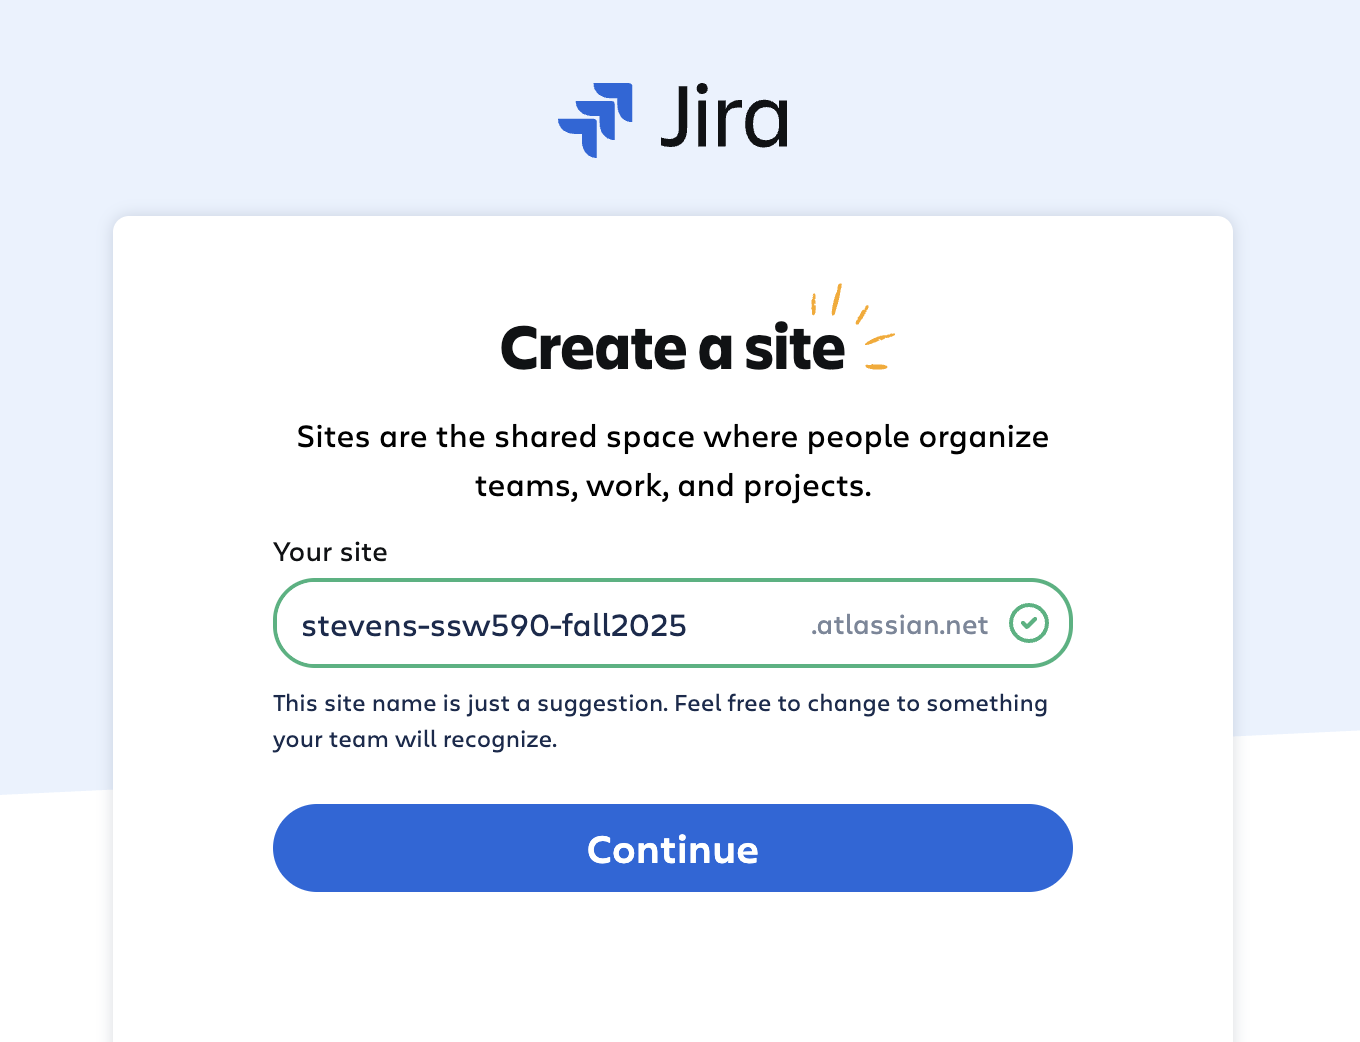
\includegraphics[width=0.7\textwidth]{png/Jira_team_setup.png}
\end{center}
I have chosen the name 'stevens-ssw590-fall2025' as the site name. \newpage

Step 2: Set up a Kanban Project 
\begin{center}
  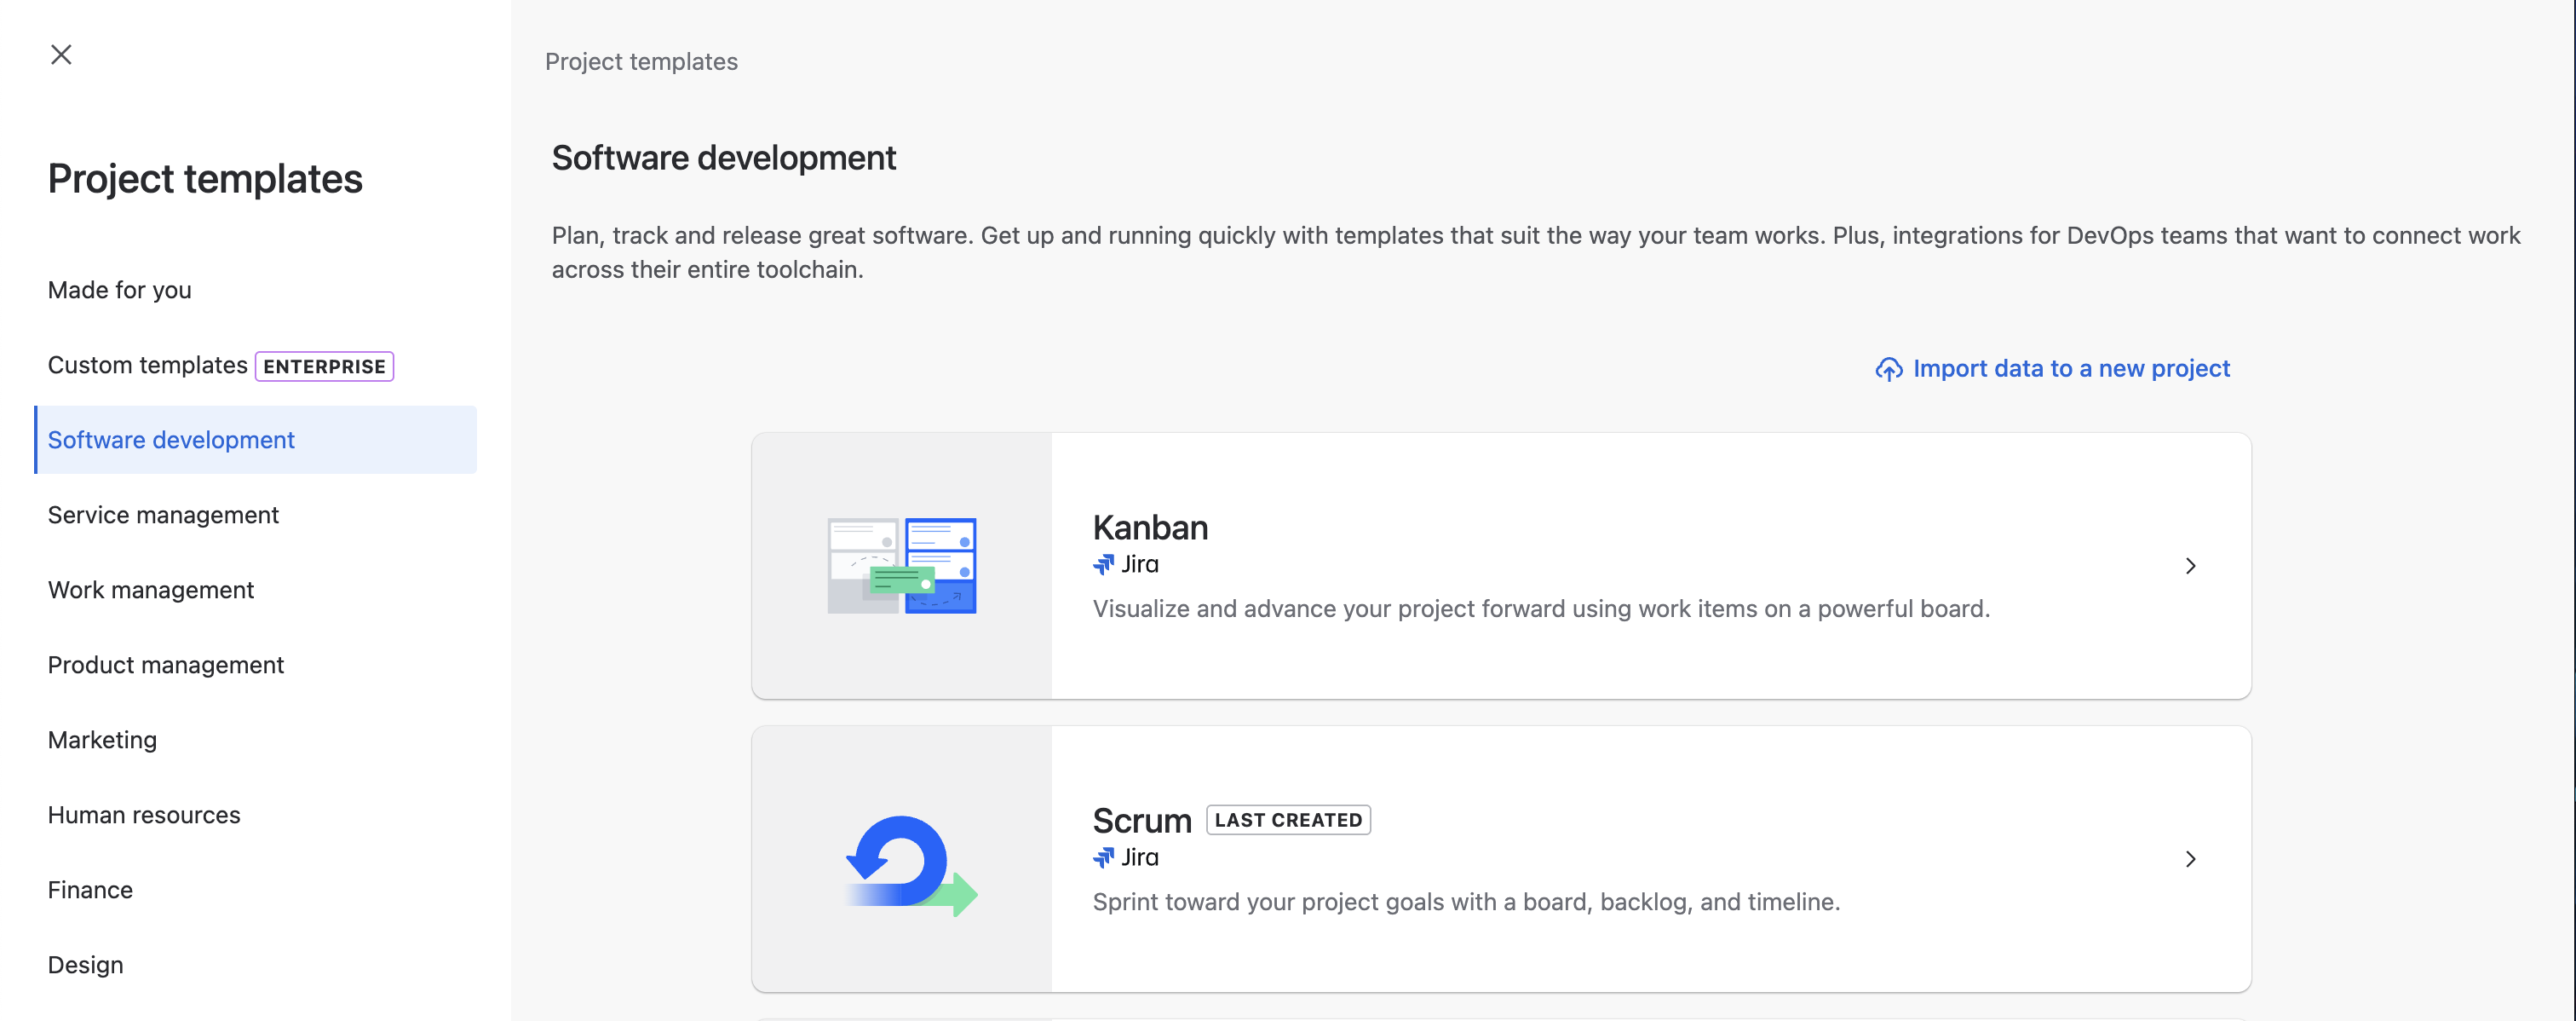
\includegraphics[width=0.9\textwidth]{png/creating_kanban_project2.png}
\end{center}

Step 3: Kanban
\begin{center}
  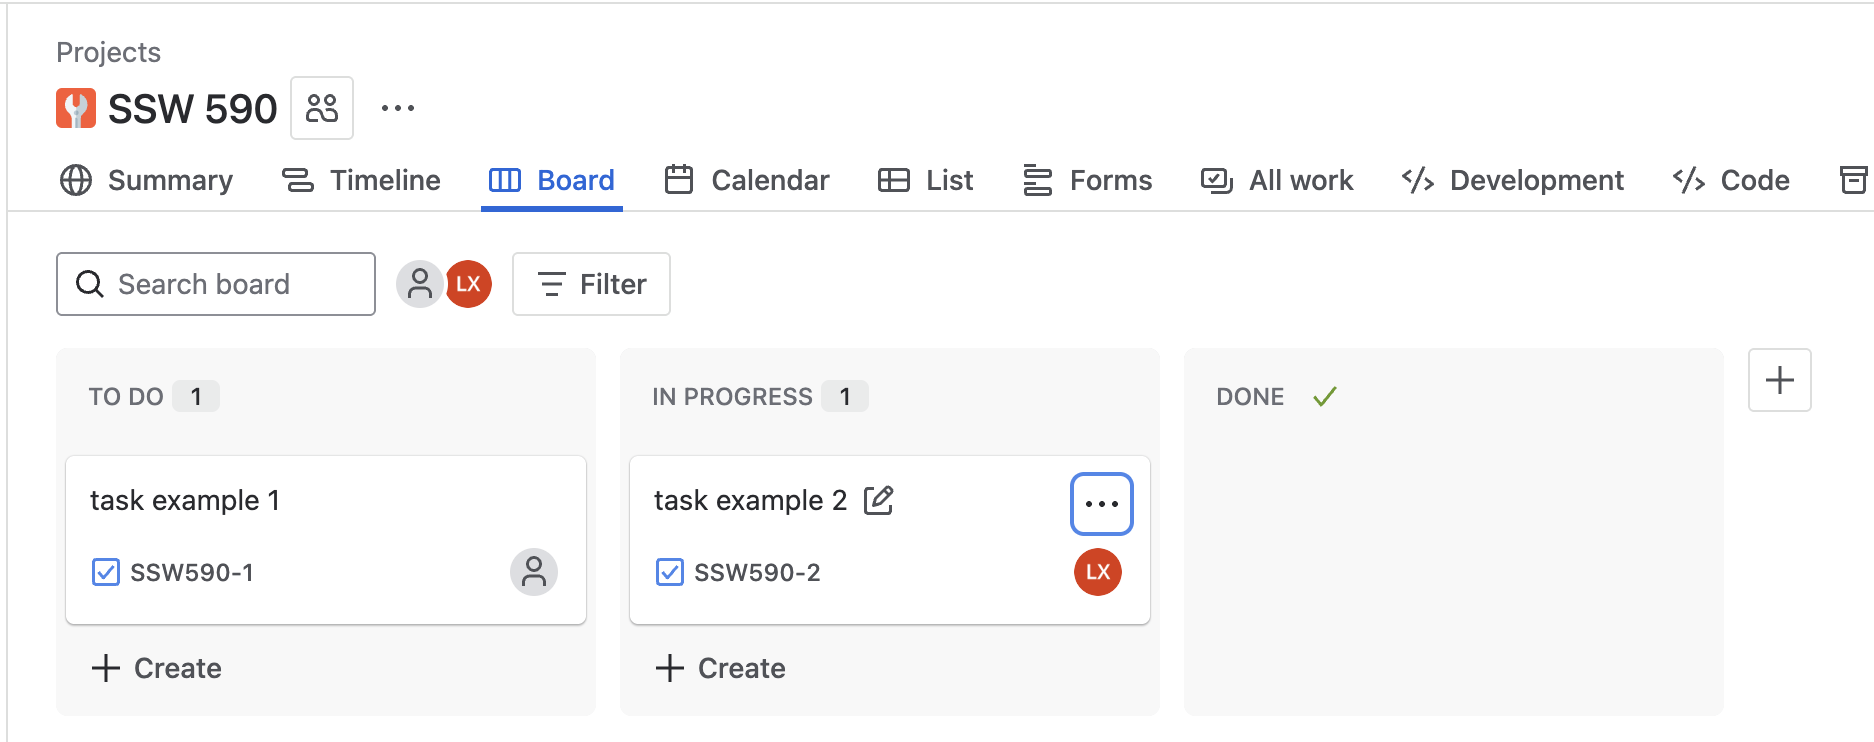
\includegraphics[width=0.9\textwidth]{png/kanban_example.png}
\end{center}
\chapter{Linux Commands \\
\small{\textit{-- Spurthi Setty, Gavin Lam, Annanya Jain, Luo Xu}}
\index{Linux Commands} 
\index{Chapter!Linux Commands}
\label{Chapter::Linux Commands}}

\section{Terminal Session}

The following commands were run from
\texttt{\~/Documents/Devops/Assignment2} and create several test files
and directories.

\begin{Verbatim}[formatcom=\color{blue}]
ubuntu@Ubuntu:~/Documents/Devops/Assignment2$ mkdir -p ~/lx-test && cd ~/lx-test
ubuntu@Ubuntu:~/lx-test$ printf "alpha\nbeta\nGamma\ngamma\nbeta\n" > words.txt
ubuntu@Ubuntu:~/lx-test$ printf "id,name,dept\n1,Ada,EE\n2,Linus,CS\n3,Grace,EE\n4,Dennis,CS\n" > people.csv
ubuntu@Ubuntu:~/lx-test$ printf "INFO boot ok\nWARN disk low\nERROR fan fail\nINFO shutdown\n" > sys.log
ubuntu@Ubuntu:~/lx-test$ dd if=/dev/zero of=blob.bin bs=1K count=48 status=none
ubuntu@Ubuntu:~/lx-test$ mkdir -p src/lib tmp archive
ubuntu@Ubuntu:~/lx-test$ printf "one two three four\n" > src/file1.txt
ubuntu@Ubuntu:~/lx-test$ printf "two three four five\n" > src/file2.txt
ubuntu@Ubuntu:~/lx-test$ ln -s src/file1.txt link-to-file1
ubuntu@Ubuntu:~/lx-test$ touch -t 202401020304 old.txt
\end{Verbatim}

\section{Problem-Set Commands and Outputs}

\subsection{Navigation \& File Ops}

\begin{enumerate}[leftmargin=2em]

  \item \textbf{Present working directory}
\begin{Verbatim}[formatcom=\color{blue}]
ubuntu@Ubuntu:~/lx-test$ pwd
/home/ubuntu/lx-test
\end{Verbatim}

  \item \textbf{List all entries, including dotfiles}
\begin{Verbatim}[formatcom=\color{blue}]
ubuntu@Ubuntu:~/lx-test$ ls -A1
archive
blob.bin
link-to-file1
old.txt
people.csv
src
sys.log
tmp
words.txt
\end{Verbatim}

  \item \textbf{Copy src/file1.txt to tmp/ only if tmp exists (verbose)}
\begin{Verbatim}[formatcom=\color{blue}]
ubuntu@Ubuntu:~/lx-test$ test -d tmp && cp -v src/file1.txt tmp/
'src/file1.txt' -> 'tmp/file1.txt'
\end{Verbatim}

  \item \textbf{Move old.txt into archive/ and keep timestamp}
\begin{Verbatim}[formatcom=\color{blue}]
ubuntu@Ubuntu:~/lx-test$ mv -v old.txt archive/
renamed 'old.txt' -> 'archive/old.txt'
\end{Verbatim}

  \item \textbf{Create an empty notes.md only if it does not exist}
\begin{Verbatim}[formatcom=\color{blue}]
ubuntu@Ubuntu:~/lx-test$ [ -e notes.md ] || : > notes.md
\end{Verbatim}

  \item \textbf{Show disk usage (human-readable) for src directory}
\begin{Verbatim}[formatcom=\color{blue}]
ubuntu@Ubuntu:~/lx-test$ du -sh src
16K    src
\end{Verbatim}


\subsection{Viewing \& Searching}

    \item \textbf{Print line numbers while displaying \texttt{sys.log}}
\begin{Verbatim}[formatcom=\color{blue}]
ubuntu@Ubuntu:~/lx-test$ nl sys.log
     1  INFO boot ok
     2  WARN disk low
     3  ERROR fan fail
     4  INFO shutdown
\end{Verbatim}

  \item \textbf{Show only the lines in \texttt{sys.log} that contain ERROR (case-sensitive)}
\begin{Verbatim}[formatcom=\color{blue}]
ubuntu@Ubuntu:~/lx-test$ grep 'ERROR' sys.log
ERROR fan fail
\end{Verbatim}

  \item \textbf{Count how many distinct words appear in \texttt{words.txt} (case-insensitive)}
\begin{Verbatim}[formatcom=\color{blue}]
ubuntu@Ubuntu:~/lx-test$ tr '[:upper:]' '[:lower:]' < words.txt | tr -s '[:space:]' '\n' | sort -u | wc -l
3
\end{Verbatim}

  \item \textbf{From \texttt{words.txt}, show lines that start with g or G}
\begin{Verbatim}[formatcom=\color{blue}]
ubuntu@Ubuntu:~/lx-test$ grep -E '^[gG]' words.txt
Gamma
gamma
\end{Verbatim}

  \item \textbf{Display the first 2 lines of \texttt{people.csv} without using an editor}
\begin{Verbatim}[formatcom=\color{blue}]
ubuntu@Ubuntu:~/lx-test$ head -n 2 people.csv
id,name,dept
1,Ada,EE
\end{Verbatim}

  \item \textbf{Show the last 3 lines of \texttt{sys.log} and keep following if the file grows}
\begin{Verbatim}[formatcom=\color{blue}]
ubuntu@Ubuntu:~/lx-test$ tail -n 3 -f sys.log
WARN disk low
ERROR fan fail
INFO shutdown
\end{Verbatim}
\subsection{Text Processing}
  \item \textbf{From people.csv, print only the name column (2nd), excluding the header.}
\begin{Verbatim}[formatcom=\color{blue}]
ubuntu@Ubuntu:~/lx-test$ tail -n +2 people.csv | cut -d',' -f2
Ada
Linus
Grace
Dennis
\end{Verbatim}

  \item \textbf{Sort words.txt case-insensitively and remove duplicates}
\begin{Verbatim}[formatcom=\color{blue}]
ubuntu@Ubuntu:~/lx-test$ sort -f words.txt | uniq -i
alpha
beta
Gamma
\end{Verbatim}

  \item \textbf{Replace every three with 3 in all files under src/ in-place, creating .bak backups.}
\begin{Verbatim}[formatcom=\color{blue}]
ubuntu@Ubuntu:~/lx-test$  find src -type f -exec sed -i.bak 's/three/3/g' {} +
\end{Verbatim}

  \item \textbf{Print the number of lines, words, and bytes for every *.txt file in src/.}
\begin{Verbatim}[formatcom=\color{blue}]
ubuntu@Ubuntu:~/lx-test$ wc src/*.txt
 1  4 15 src/file1.txt
 1  4 16 src/file2.txt
 2  8 31 total
\end{Verbatim}

\subsection{Permissions \& Ownership}

  \item \textbf{Make tmp/ readable, writable, and searchable only by the owner.}
\begin{Verbatim}[formatcom=\color{blue}]
ubuntu@Ubuntu:~/lx-test$ chmod 700 tmp/

\end{Verbatim}

  \item \textbf{Give group execute permission to src/lib recursively without touching others/owner bits.}
\begin{Verbatim}[formatcom=\color{blue}]
ubuntu@Ubuntu:~/lx-test$ chmod -R g+x src/lib
\end{Verbatim}

  \item \textbf{Show the numeric (octal) permissions of src/file2.txt}
\begin{Verbatim}[formatcom=\color{blue}]
ubuntu@Ubuntu:~/lx-test$ stat -c "%a" src/file2.txt
664
\end{Verbatim}

  \item \textbf{Make notes.md append-only for the owner via file attributes (if supported).}
\begin{Verbatim}[formatcom=\color{blue}]
ubuntu@Ubuntu:~/lx-test$ sudo chattr +a notes.md
\end{Verbatim}

\subsection{Links \& Find}

\item \textbf{Verify whether link-to-file1 is a symlink and show its target path.}
\begin{Verbatim}[formatcom=\color{blue}]
luo@ubuntuluo:~/lx-test$ ls -l link-to-file1
lrwxrwxrwx 1 luo luo 13 Sep 16 18:56 link-to-file1 -> src/file1.txt
\end{Verbatim}

\item \textbf{Find all regular files under the current tree larger than 40 KiB.}
\begin{Verbatim}[formatcom=\color{blue}]
luo@ubuntuluo:~/lx-test$ find . -type f -size +40k
\end{Verbatim}

\item \textbf{Find files modified in the last 10 minutes under tmp/ and print their sizes.}
\begin{Verbatim}[formatcom=\color{blue}]
luo@ubuntuluo:~/lx-test$ find tmp/ -type f -mmin -10 -exec ls -lh {} +
\end{Verbatim}

\subsection{Processes \& Job Control}

\item \textbf{Show your processes in a tree view.}
\begin{Verbatim}[formatcom=\color{blue}]
luo@ubuntuluo:~/lx-test$ pstree -p
\end{Verbatim}

\item \textbf{Start sleep 120 in the background and show its PID.}
\begin{Verbatim}[formatcom=\color{blue}]
luo@ubuntuluo:~/lx-test$ sleep 120 &
echo $!
[1] 4474
4474

\end{Verbatim}

\item \textbf{Send a TERM signal to all sleep processes owned by you (don’t use kill -9).}
\begin{Verbatim}[formatcom=\color{blue}]
luo@ubuntuluo:~/lx-test$ pkill -TERM -u "$USER" sleep

[1]  + Terminated  sleep 120

\end{Verbatim}

\item \textbf{Show the top 5 processes by memory usage (one-shot, not interactive).}
\begin{Verbatim}[formatcom=\color{blue}]
luo@ubuntuluo:~/lx-test$ ps -eo pid,ppid,user,%mem,%cpu,comm --sort=-%mem | head -n 5
PID    PPID USER     %MEM %CPU COMMAND
   1925    1711 luo       9.8  4.0 gnome-shell
   2451    1925 luo       2.4  0.0 mutter-x11-fram
   2328    1711 luo       2.0  0.0 gsd-xsettings
   2245    1925 luo       1.7  0.0 Xwayland

\end{Verbatim}

\subsection{Archiving \& Compression}

\item \textbf{Create a gzipped tar archive src.tgz from src/ with relative paths.}
\begin{Verbatim}[formatcom=\color{blue}]
luo@ubuntuluo:~/lx-test$ tar -czf src.tgz -C src .
\end{Verbatim}

\item \textbf{List the contents of src.tgz without extracting.}
\begin{Verbatim}[formatcom=\color{blue}]
luo@ubuntuluo:~/lx-test$ tar -tzf src.tgz
./
./file2.txt
./lib/
./file1.txt.bak
./file2.txt.bak
./file1.txt

\end{Verbatim}

\item \textbf{Extract only file2.txt from src.tgz into tmp/.}
\begin{Verbatim}[formatcom=\color{blue}]
luo@ubuntuluo:~/lx-test$ tar -xvzf src.tgz -C tmp ./file2.txt
./file2.txt

\end{Verbatim}

\subsection{Networking \& System Info}

\item \textbf{Show all listening TCP sockets with associated PIDs (no root assumptions).}
\begin{Verbatim}[formatcom=\color{blue}]
annanyajain@ubuntu:-/lx-test$ ss -tlnp
State   Recv-Q   Send-Q     Local Address:Port     Peer Address:Port  Process 
\end{Verbatim}

\item \textbf{Print your default route (gateway) in a concise form.}
\begin{Verbatim}[formatcom=\color{blue}]
annanyajain@ubuntu:-/lx-test$ ip route show default
default via 198.19.249.1 dev eth0 proto dhcp src 198.19.249.228 metric 100 
\end{Verbatim}

\item \textbf{Display kernel name, release, and machine architecture.}
\begin{Verbatim}[formatcom=\color{blue}]
annanyajain@ubuntu:-/lx-test$ uname -srm
Linux 6.12.10-orbstack-00297-gf8f6e015b993 aarch64
\end{Verbatim}

\item \textbf{Show the last 5 successful logins (or last sessions) on the system.}
\begin{Verbatim}[formatcom=\color{blue}]
annanyajain@ubuntu:-/lx-test$ last -n 5
reboot   system boot  6.12.10-orbstack Tue Sep 16 01:01   still running
reboot   system boot  6.12.10-orbstack Tue Jan 21 13:27 - 13:40  (00:12)
reboot   system boot  6.12.10-orbstack Tue Jan 21 10:51 - 10:56  (00:04)
reboot   system boot  6.12.9-orbstack- Mon Jan 20 19:48 - 19:48  (00:00)
reboot   system boot  6.12.9-orbstack- Mon Jan 20 17:30 - 19:48  (02:18)

wtmp begins Mon Jan 20 15:07:29 2025
\end{Verbatim}


\subsection{Package \& Services (Debian/Ubuntu)}

\item \textbf{Show the installed version of package coreutils.}
\begin{Verbatim}[formatcom=\color{blue}]
annanyajain@ubuntu:-/lx-test$ dpkg -s coreutils | grep '^Version:'
Version: 8.32-4.1ubuntu1.2

\end{Verbatim}

\item \textbf{Search available packages whose names contain ripgrep.}
\begin{Verbatim}[formatcom=\color{blue}]
annanyajain@ubuntu:-/lx-test$ apt search ripgrep
Sorting... Done
Full Text Search... Done
elpa-dumb-jump/jammy 0.5.3-1 all
  jump to definition for multiple languages without configuration

ripgrep/jammy-updates,jammy-security 13.0.0-2ubuntu0.1 arm64
  Recursively searches directories for a regex pattern

ugrep/jammy 3.7.2+dfsg-1 arm64
  faster grep with an interactive query UI

\end{Verbatim}

\item \textbf{Check whether service cron is active and print its status line only.}
\begin{Verbatim}[formatcom=\color{blue}]
annanyajain@ubuntu:-/lx-test$ systemctl status cron | grep 'Active:'
     Active: active (running) since Tue 2025-09-16 01:01:18 EDT; 31min ago

\end{Verbatim}


\subsection{Bash \& Scripting}

\item \textbf{Write a one-liner that loops over *.txt in src/ and prints: : (Let's print number of words in the files)}
\begin{Verbatim}[formatcom=\color{blue}]
annanyajain@ubuntu:-/lx-test$ for f in src/*.txt; do echo "$f: $(wc -w < "$f")";done
src/file1.txt: 4
src/file2.txt: 4

\end{Verbatim}


\item \textbf{Write a command that exports CSV rows where dept == "CS" to cs.txt (exclude header)}.

\text{So here, let me first see the structure of a csv file in src directory:}

\begin{Verbatim}[formatcom=\color{blue}]
annanyajain@ubuntu:-/lx-test$ cat people.csv
id,name,dept
1,Ada,EE
2,Linus,CS
3,Grace,EE
4,Dennis,CS

\end{Verbatim}

\text{Now I know that third column is the dept:}

\begin{Verbatim}[formatcom=\color{blue}]
annanyajain@ubuntu:-/lx-test$ awk -F, 'NR>1 && $3=="CS" {print}' people.csv > cs.txt
\end{Verbatim}

\text{The output is redirected into the cs.txt file. We can now verify the results:}

\begin{Verbatim}[formatcom=\color{blue}]
annanyajain@ubuntu:-/lx-test$  cat cs.txt
2,Linus,CS
4,Dennis,CS
\end{Verbatim}


\item \textbf{Create a variable X with value 42, print it, then remove it from the environment.
}
\begin{Verbatim}[formatcom=\color{blue}]
annanyajain@ubuntu:-/lx-test$ export X=42; echo $X; unset X
42

\end{Verbatim}
The variable X was created with value 42, and printed. The bash command (unset X) was used to remove it from the environment. Now, let's verify whether the variable is still there:

\begin{Verbatim}[formatcom=\color{blue}]
annanyajain@ubuntu:-/lx-test$ echo $X;

\end{Verbatim}
\text{Nothing got printed. Hence, it is removed from the environment.}

\end{enumerate}
\chapter{Project Proposal \\
\small{\textit{-- Luo Xu, Annanya Jain, Gavin Lam}}
\index{Project Proposal} 
\index{Chapter!Project Proposal}
\label{Chapter::Project Proposal}}

Our project is an AI Health Voice Assistant named AVA, short for Artificial Voice Assistant. Users will be able to log in and create an account and chat with AVA. This project aims to support users in tracking emotions, managing reminders, and accessing mental wellness resources. Unlike traditional chatbots, our assistant goes beyond simple question–answer interaction by integrating:

\begin{itemize}
\item Agentic AI workflows, enabling the assistant to interpret user intent, plan actions, and decide between generating responses, retrieving wellness exercises, or scheduling reminders.

\item DevSecOps practices to make it scalable, and secure from development to deployment.
The end goal is a functional prototype that not only demonstrates AI-driven health support but also serves as a practical use of modern DevOps pipelines and monitoring
\end{itemize} 
This project will be an enhancement of our previously created project for CS555 course. Since then we have grown a lot in terms of knowledge and skill sets and we would like to improve it to have agentic powers 
to better aid users. Here is the link for the repository for the project: 
\url{https://github.com/cascadingluo/SSW590-team-7-project}

\begin{longtable}{|p{4cm}|p{10cm}|}
\hline
\textbf{Tool} & \textbf{Usage} \\ \hline
Flask & Web framework. \\ \hline
MongoDB & Database for user information and chat history storage. \\ \hline
Gemini & AI API used for the chatbot. \\ \hline
GitHub & Source Control and Collaboration \\ \hline
CI/CD & Github Actions for automated testing\\ \hline
Jira & Issue tracking and Agile project management tool. \\ \hline
AWS & Pushing local Docker with AWS and deploying with App Runner. \\ \hline
TikZ & Vizualizing Architecture of our assistant. \\ \hline 
\end{longtable}
 
\chapter{AWS \\
\small{\textit{-- Gavin Lam, Luo Xu, Annanya Jain}
\index{AWS} 
\index{Chapter!AWS}
\label{Chapter::AWS}}}

To get our website deployed, we followed the steps in the DockerLocalAndAWS.pdf document with some changes to the code as parts in the document did not work on our machines.\medskip

\noindent First we created an AWS root account at \textcolor{blue}{aws.amazon.com}. MFA was enabled on the root account and our region was set to us-east-2. A cost budget was set up as well to monitor costs. The SSO start URL was also recorded to be used later\medskip

\noindent We then enabled the IAM Identity center and created a new user with an alternate email. At first this user wasn't able to access any dashboards at it had no roles or permissions. This user was given the permission set AdministratorAccess by the root account and after a relog was able to access a dashboard. From this dashboard the AWS Access Key ID, AWS Secret Access Key, and AWS session ID were written down. \medskip

\noindent After the AWS accounts were correctly set up, we ran the commands in the document on the terminal.
\begin{minted}{shell}
aws configure sso
\end{minted}

\noindent This command prompted us to give answers

\begin{minted}{shell}
#SSO session name:
#SSO start URL:
#SSO region:
#Account:
#Role:
#Default region:
#Output:
\end{minted}

\noindent After entering all the details the login were saved.

The command ran next was 

\begin{minted}{shell}
aws configure 
\end{minted}

\noindent This command prompted us to give answers

\begin{minted}{shell}
#AWS Access key ID:
#AWS Secret Access key:
#AWS Session ID:
#Default region:
#Output:
\end{minted}

\noindent After entering all the details we successfully logged in and ran another command to confirm.

\begin{minted}{shell}
aws sts get-caller-identity
\end{minted}

\noindent The next steps were to create an ECR repository as stated in the document. We first set some environment variables through these commands.

\begin{minted}{shell}
export AWS_REGION=us-east-2
export ECR_REPO=myapp
export IMAGE_TAG=v1
export CONTAINER_PORT=3000
export AWS_ACCOUNT_ID="$(aws sts get-caller-identity --query Account --output text --profile (my account here))"
\end{minted}

\noindent After setting the variables we created a new ECR repository through these commands.

\begin{minted}{shell}
aws ecr create-repository \
    --repository-name "$ECR_REPO" \
    --image-scanning-configuration scanOrPush=true \
    --region "AWS_REGION" --profile (my account here)
\end{minted}

\noindent AWS CLI was then used to obtain a short-lived registry token and logged in Docker.

\begin{minted}{shell}
aws ecr get-login-password --region "$AWS_REGION" --profile default \
| docker login --username AWS --password-stdin \
    "$AWS_ACCOUNT_ID.dkr.ecr.$AWS_REGION.amazonaws.com"
\end{minted}

\noindent Our local image was then built, tagged, and pushed. These commands were run from the directory containing the Dockerfile.

\begin{minted}{shell}
docker build --platform linux/amd64 -t "$ECR_REPO:$IMAGE_TAG" .

docker tag "$ECR_REPO:$IMAGE_TAG" \
"$AWS_ACCOUNT_ID.dkr.ecr.$AWS_REGION.amazonaws.com/$ECR_REPO:$IMAGE_TAG"

docker push "$AWS_ACCOUNT_ID.dkr.ecr.$AWS_REGION.amazonaws.com/$ECR_REPO:$IMAGE_TAG"
\end{minted}

\noindent Verifying the image in ECR was next


\begin{minted}{shell}
aws ecr describe-images \
    --repository-name "$ECR_REPO" \
    --region "$AWS_REGION" --profile default \
    --query 'imageDetails[].imageTags'
\end{minted}

\noindent The next step of quick deploying with App Runner was where we ran into a roadblock. The code shown when inputted resulted in the error below. 


\begin{minted}{shell}
export APP_NAME=my-apprunner-app

aws apprunner create-service \
    --service-name "$APP_NAME" \
    --region "$AWS_REGION" --profile default \
    --source-configuration "{
        \"ImageRepository\": {
            \"ImageIdentifier\": \"$AWS_ACCOUNT_ID.dkr.ecr.$AWS_REGION.amazonaws.com/$ECR_REPO:$IMAGE_TAG\",
            \"ImageRepositoryType\": \"ECR\",
            \"ImageConfiguration\": {\"Port\": \"$CONTAINER_PORT\"}
    },
\"AutoDeploymentsEnabled\": true
}" \
--instance-configuration "{\"Cpu\":\"1 vCPU\",\"Memory\":\"2 GB\"}"
\end{minted}

\begin{minted}{shell}
An error occurred (InvalidRequestException) when calling the CreateService operation: Authentication configuration is invalid.
\end{minted}

\noindent After looking at online resources we assumed that the permission set AdministratorAccesss was not working as we hoped and didn't give us the permissions we needed to use CreateService. In order to fix this we created a trust policy named AppRunnerECRAccessRole in IAM roles. The json used is:

\begin{minted}{JSON}
{ "Version": "2012-10-17", 
    "Statement": [ 
    { 
      "Effect": "Allow", 
      "Action": "iam:PassRole", 
      "Resource": "arn:aws:iam::(our account id here):role/AppRunnerECRAccessRole" 
    }, 
    { 
      "Effect": "Allow", 
      "Action": [ "apprunner:CreateService", "apprunner:UpdateService", 
      "apprunner:DeleteService" ], 
      "Resource": "*" } 
    ] 
}

\end{minted}

\noindent After relogging the SSO session and rerunning early commands to confirm we are logged in properly everywhere we retried the original deploying command again. We did some more research and found out more commands we could try. First we had to update the trust policy to replace the second bracket of code. 

\begin{minted}{JSON}
{
  "Version": "2012-10-17",
  "Statement": [
    {
      "Effect": "Allow",
      "Principal": { "Service": "build.apprunner.amazonaws.com" },
      "Action": "sts:AssumeRole"
    }
  ]
}

\end{minted}

\noindent The final inline policy we used is

\begin{minted}{JSON}
{
  "Version": "2012-10-17",
  "Statement": [
    { 
      "Effect": "Allow", 
      "Action": "iam:PassRole", 
      "Resource": "arn:aws:iam::(our account id here):role/AppRunnerECRAccessRole" 
    }, 
    {
      "Effect": "Allow",
      "Principal": { "Service": "build.apprunner.amazonaws.com" },
      "Action": "sts:AssumeRole"
    }
  ]
}

\end{minted}


\noindent We then had to attach permissions to the role. The AWS managed policy AWSAppRunnerServicePolicyForECRAccess was added. After confirming the role we retried the command again. The error persisted. We were stuck at this point so we prompted chatGPT multiple times before it recommended us to correct the create-service command with safe quoting, i.e. use single quotes around the JSON blocks so the shell does not break the quoting. The new create-service command is

\begin{minted}{shell}
aws apprunner create-service \
  --service-name "$APP_NAME" \
  --region "$AWS_REGION" --profile default \
  --source-configuration '{
    "ImageRepository": {
      "ImageIdentifier": "'"$AWS_ACCOUNT_ID"'.dkr.ecr.'"$AWS_REGION"'.amazonaws.com/'"$ECR_REPO"':'"$IMAGE_TAG"'",
      "ImageRepositoryType": "ECR",
      "ImageConfiguration": { "Port": "'"$CONTAINER_PORT"'" }
    },
    "AuthenticationConfiguration": {
      "AccessRoleArn": "arn:aws:iam::'"$AWS_ACCOUNT_ID"':role/AppRunnerECRAccessRole"
    },
    "AutoDeploymentsEnabled": true
  }' \
  --instance-configuration '{
    "Cpu": "1 vCPU",
    "Memory": "2 GB"
  }'


\end{minted}

\noindent This miraculously went through, and we thought we had successfully created the service. We continued following the steps in the document creating more environment variables. 

\begin{minted}{shell}
AWS_REGION=us-east-2
PROFILE=(Our Profile here)
SERVICE_ARN=(Our Servive ARN here)
  }


\end{minted}

\noindent We then tried to run the service status changes to running command but this resulted in another error:

\begin{minted}{shell}

while true; do
STATUS=$(aws apprunner describe-service \
--service-arn "$SERVICE_ARN" \
--region "$AWS_REGION" --profile "$PROFILE" \
--query 'Service.Status' --output text)
echo "Service status: $STATUS"
case "$STATUS" in RUNNING|CREATE_FAILED|OPERATION_FAILED) break ;; esac
sleep 4
done


\end{minted}

\begin{minted}{shell}

An error occurred (InvalidRequestException) when calling the DescribeService operation: Authentication configuration is invalid.


\end{minted}

\noindent We then read the document again and saw that the next line was to grab the service URL and just hoped that the service was running properly. 

\begin{minted}{shell}

aws apprunner list-services \
--region "$AWS_REGION" --profile default \
--query "ServiceSummaryList[?ServiceName=='$APP_NAME'].ServiceUrl" --output text

\end{minted}


\noindent Unfortunately, it did not create successfully and we ran into an error website. We were stuck at this point and did not know how to proceed so we decided to leave it for a little bit and come back at a later time to retry. \medskip

\noindent After coming back at a later time we reran through the steps of, aws configure sso, aws configure (with new details this time), sanity test, resetting the environment variables (they did not change from above we just reentered them), authenticated Docker to ECR, built, tagged, and pushed the local image, verified the image in ECR, deployed with App Runner. This is where we ran into the same error, but we found a service on AWS called CloudWatch that essentially replaced the need for the "test the service status changes to running" command. CloudWatch enabled us to look at the logs of services we have tried to deploy. After checking CloudWatch we saw the previous instance of our service had failed due to the ECR repository not being recognized, and saw that our most recent creation of the service had successfully deployed. We then ran the command to get the service URL.


\begin{minted}{shell}

aws apprunner list-services \
--region "$AWS_REGION" --profile default \
--query "ServiceSummaryList[?ServiceName=='$APP_NAME'].ServiceUrl" --output text

\end{minted}

\noindent Which resulted in

\begin{minted}{shell}

mu3fbjbbv2.us-east-2.awsapprunner.com

\end{minted}

\noindent This URL works, which means our deployment with AWS was successful.


\noindent After the successful deployment, we change the code for the original website to use a class-based javascript code instead of methods. The code largely remain the same, we just moved parts of code in the html file into a javascript file and had the html file run the script instead of the code directly. We have the new ColorController class that has DOM references, event binding and the color-changing behaviors. ColorController.init() connects the app on DOMContentLoaded. Here is the code in our new javascript file:

\begin{minted}{javascript}
class ColorController { //class 
  constructor({ blueBtnId = "blueBtn", redBtnId = "redBtn", target = document.body } = {}) {
    this.target = target;
    this.blueBtn = document.getElementById(blueBtnId);
    this.redBtn  = document.getElementById(redBtnId);
    this._bind();
  }

  // private method to bind event listeners, the same exact code as the ones originally in html
  _bind() {
    if (this.blueBtn) {
      this.blueBtn.addEventListener("click", () => this.setColor("blue"));
    }
    if (this.redBtn) {
      this.redBtn.addEventListener("click", () => this.setColor("red"));
    }
  }

  setColor(color) {
    this.target.style.backgroundColor = color;
  }

  static init(opts) {
    return new ColorController(opts);
  }
}

document.addEventListener("DOMContentLoaded", () => {
  ColorController.init();
});

\end{minted}

Here is the UML diagram for the new code (this was created with the help of GPT-5):

\begin{minted}[fontsize=\small]{text}
+-------------------+
|   ColorController |
+-------------------+
| - blueBtn: Button |
| - redBtn:  Button |
| - target: Element |
+-------------------+
| + constructor(...)|
| - _bind(): void   |
| + setColor(c):void|
| + init(...): CC   |
+-------------------+

Notes:
- constructor wires DOM elements and calls _bind()
- _bind attaches event listeners to blue/red buttons
- setColor updates the background color of the target
- init is a convenience factory method
\end{minted}

\chapter{LaTeX Docker \\
\small{\textit{-- Annanya Jain, Gavin Lam, Luo Xu}
\index{LaTeX Docker} 
\index{Chapter!LaTeX Docker}
\label{Chapter::LaTeX Docker}}}


In this chapter, we created a Docker container to compile a simple LaTeX document using TeX Live, which is basically what Overleaf does. \medskip

\section{Steps taken for creating the docker container to compile a LaTeX File}

I created the following files in a folder named: texlive-app:

\begin{minted}{text}
texlive-app/
├── Dockerfile
└── main
\end{minted}

\subsection{main.tex}

\begin{minted}{latex}

\begin{document}

\title{Password Policy Documentation}
\date{\today}
\maketitle
Let me take an example of LaTeX file with a simple table to compile. 
\section{Password Rules}
\begin{longtable}{|l|p{9cm}|} 
\caption{Password Rules \label{Table::Passwords}}\\
\hline
\textbf{User} & \textbf{Password Rule / Hint} \\
\hline
\endhead

devuser & At least 8 characters, include uppercase, 
lowercase, a number, and a symbol. Hint: First pet. 
\\ 
\hline

admin & Must change passwords every 90 days. Hint: Favorite City. 
\\ 
\hline

tester & Must include word banana Hint: Popular dessert item. 
\\ 
\hline

\end{longtable}

\end{document}
\end{minted}

\subsection{Dockerfile}
\begin{minted}{docker}
FROM debian:stable-slim

RUN apt-get update && apt-get install -y \
    texlive-latex-base \
    texlive-latex-recommended \
    texlive-latex-extra \
    texlive-fonts-recommended \
    texlive-fonts-extra \
    && rm -rf /var/lib/apt/lists/*

WORKDIR /data

CMD ["pdflatex", "main.tex"]
\end{minted}

\subsection{Building the Docker image}
To build and run the container:

\begin{minted}{bash}
docker build -t texlive-app .
docker run --rm -v $(pwd):/data texlive-app
\end{minted}

\begin{center}
  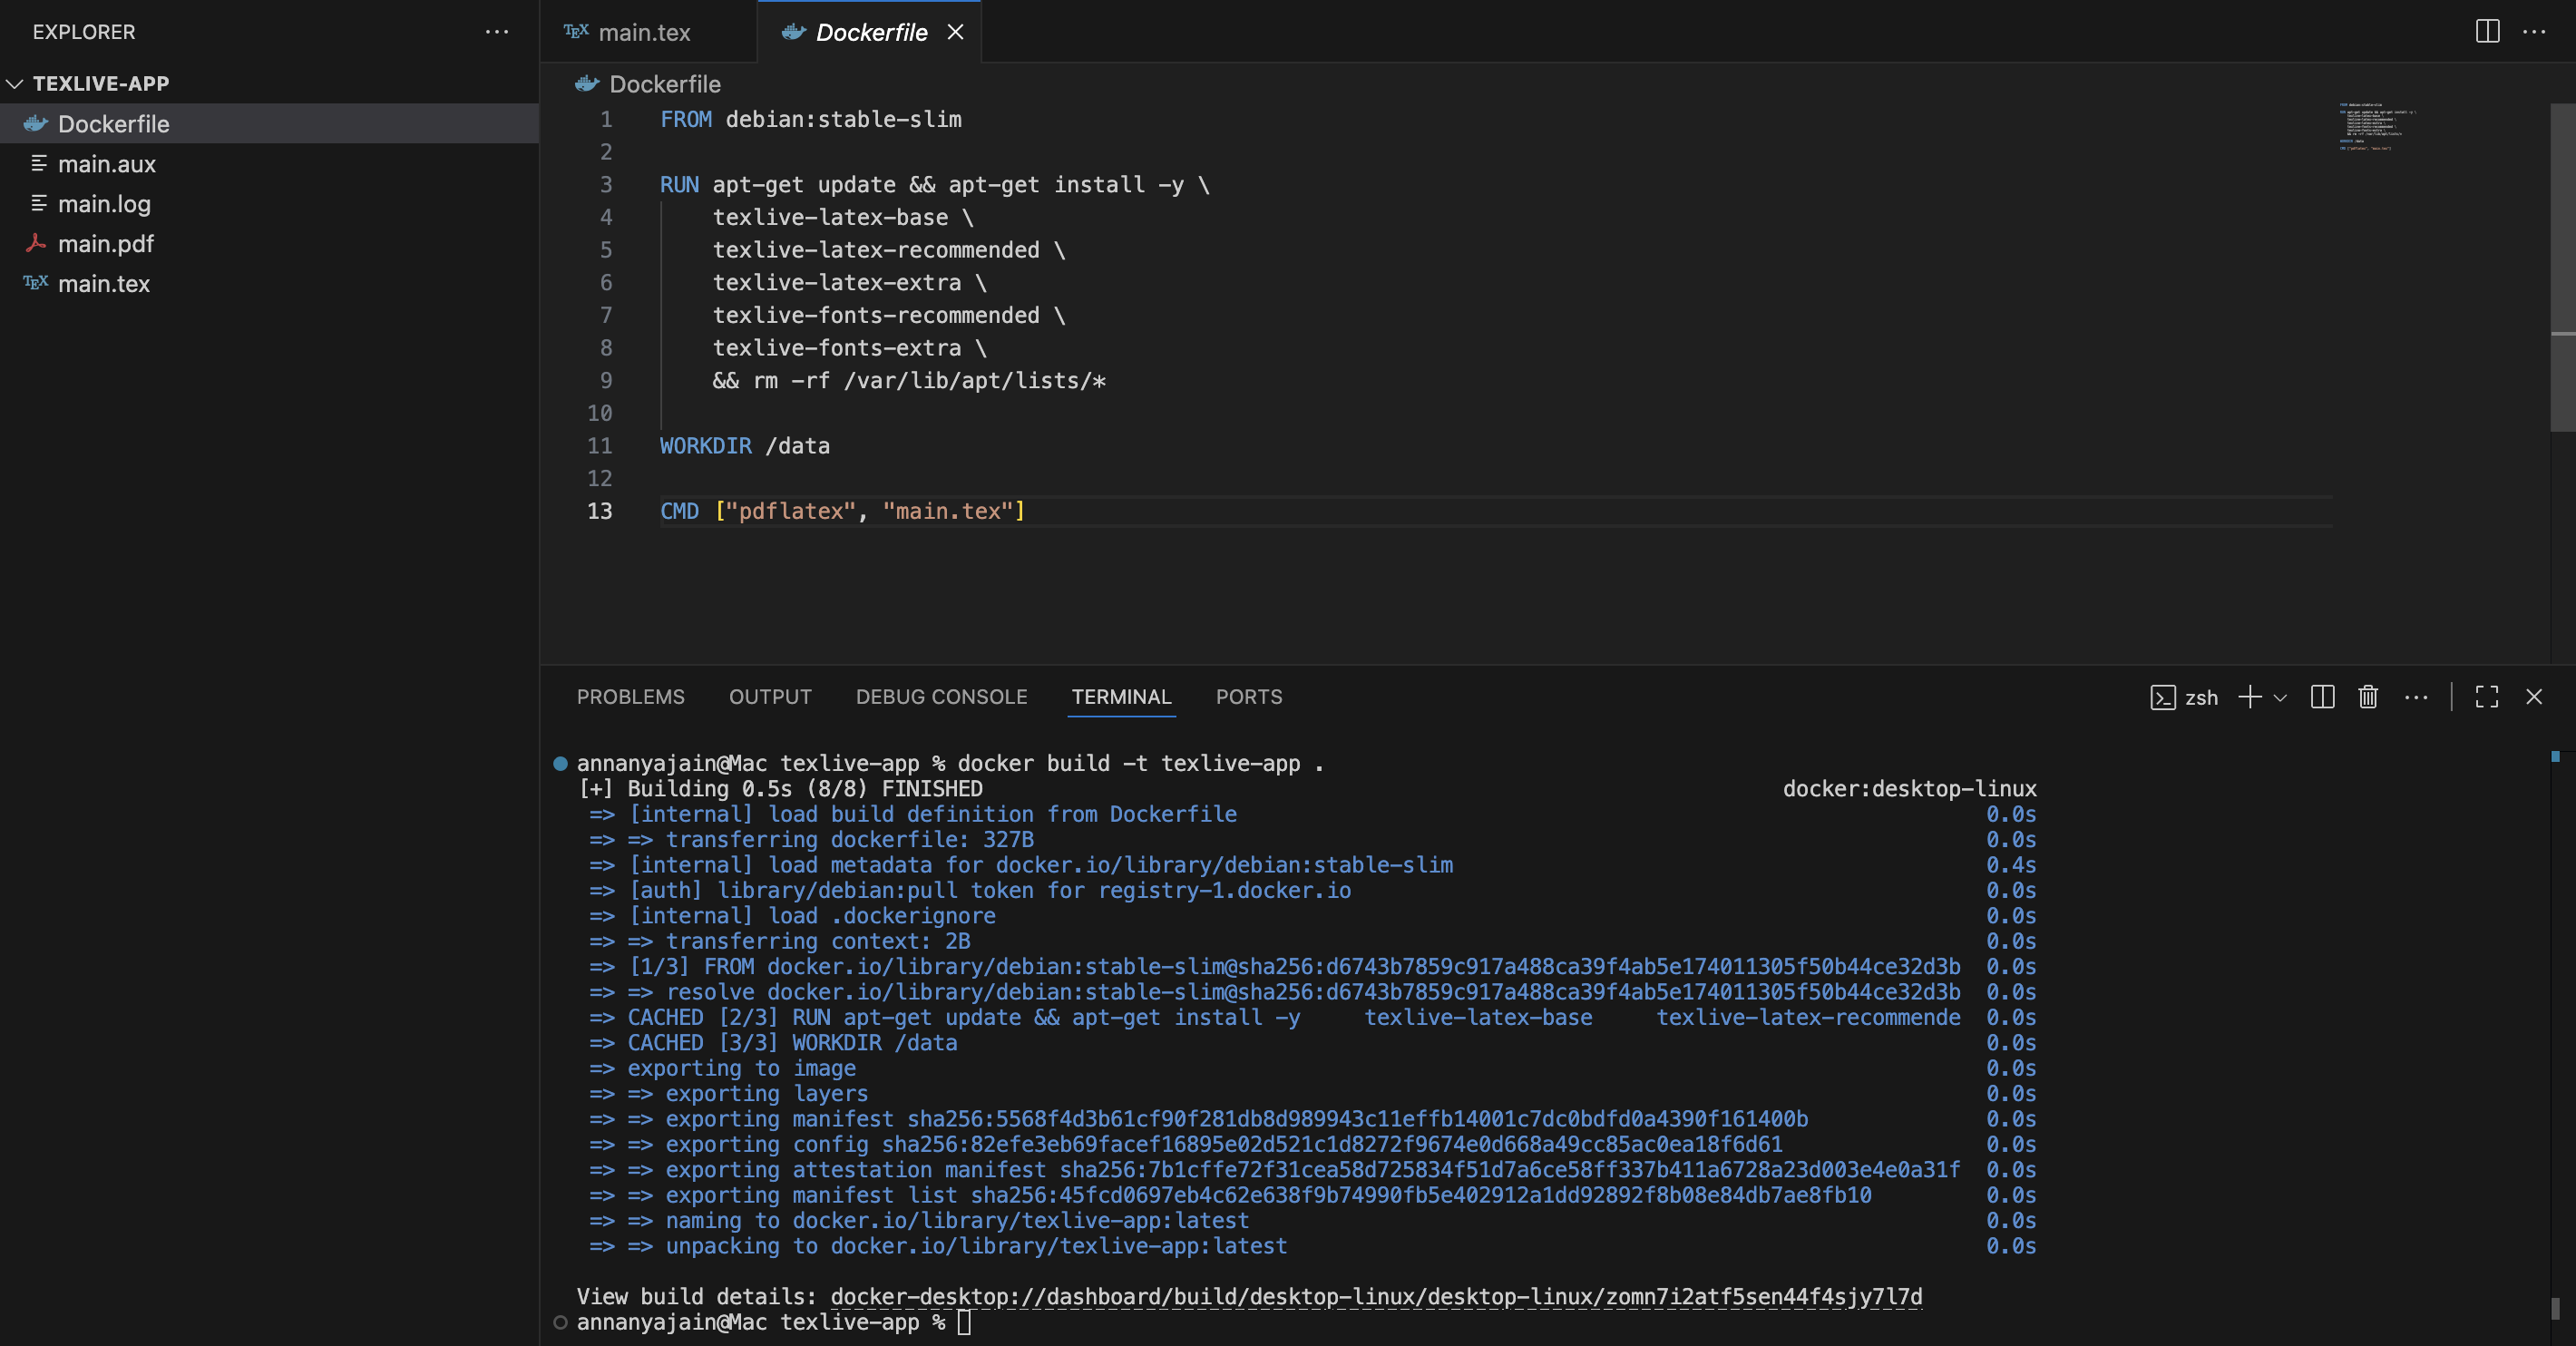
\includegraphics[width=1.0\textwidth]{png/texlive_build.png}
\end{center}

\noindent After running the commands, the output file \texttt{main.pdf} 
gets generated in the project folder on the machine. \medskip

\begin{center}
  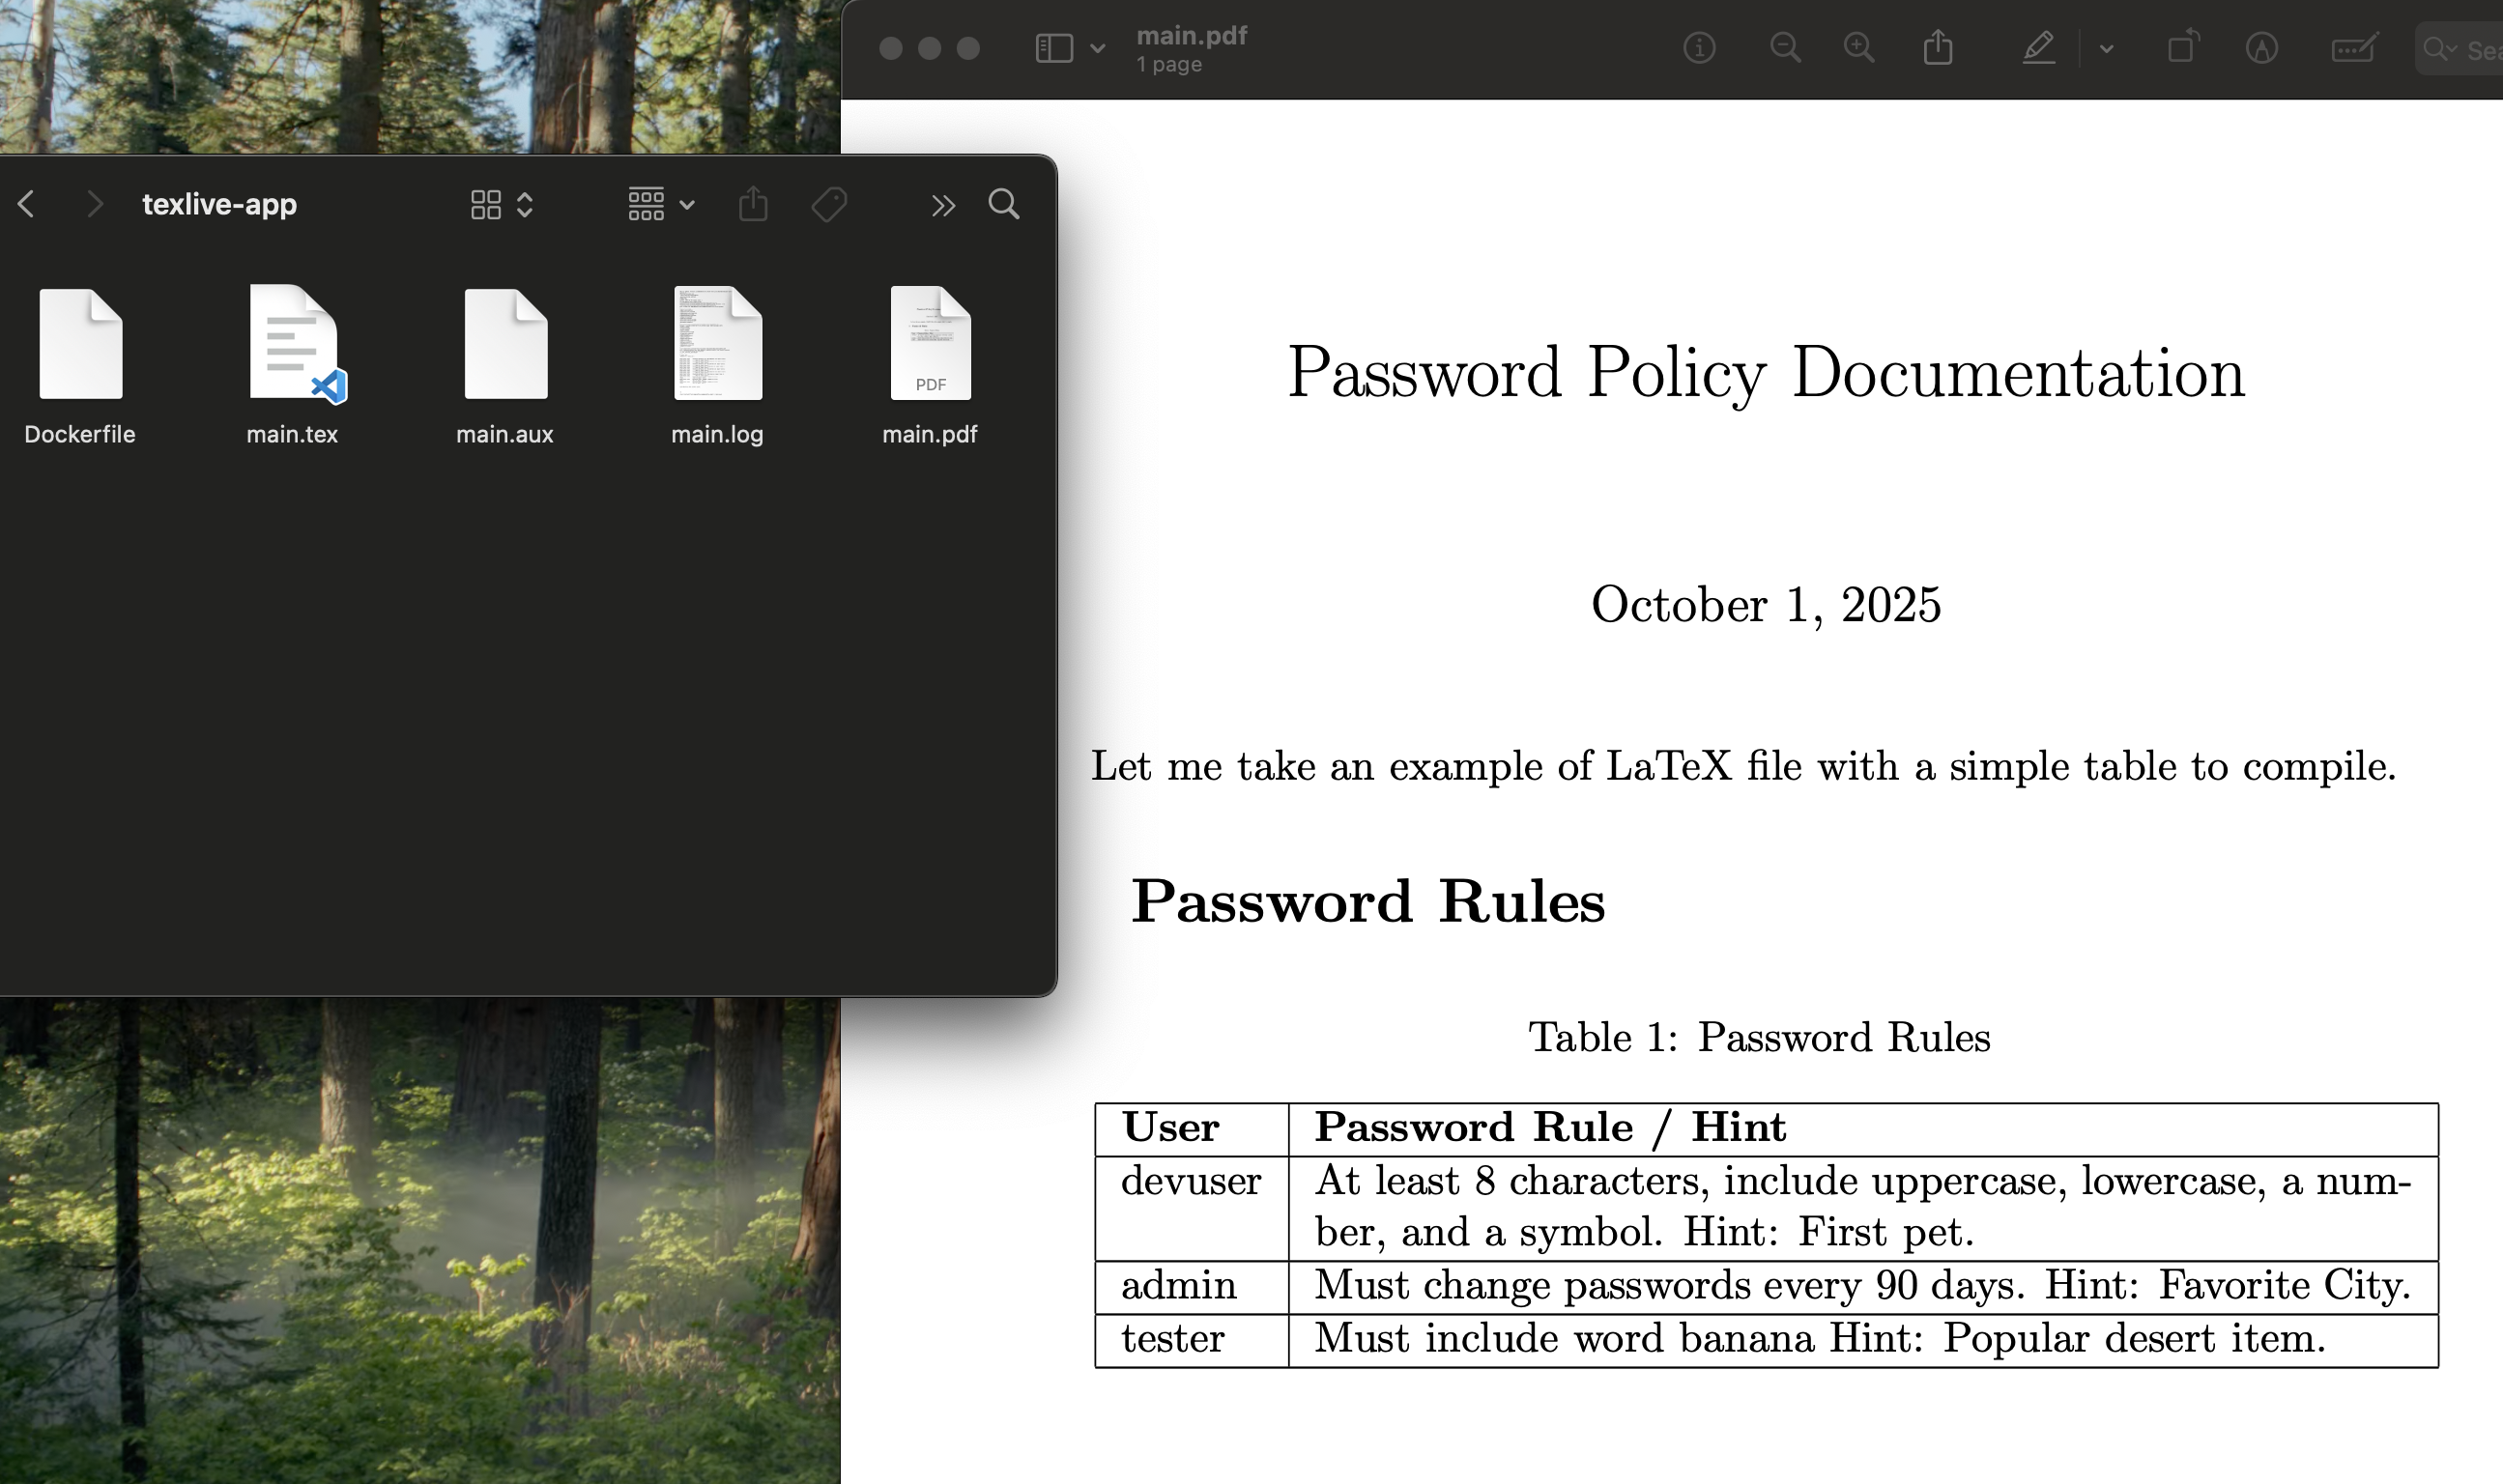
\includegraphics[width=1.0\textwidth]{png/main_pdf generated.png}
\end{center}



\chapter{Bugzilla \\
\small{\textit{-- Luo Xu, Gavin Lam, Annanya Jain}
\index{Bugzilla} 
\index{Chapter!Bugzilla}
\label{Chapter::Bugzilla}}}

\section{DigitalOcean Setup}
We made an account in DigitalOcean via GitHub and received 200 credits via student package.

\noindent We created an droplet with these stats: 2 GB Memory / 60 GB Disk / NYC3 - Ubuntu 24.04 (LTS) x64

\section{Bugzilla}
After setting up the droplet, we ssh into the droplet through the local terminal with the public ip: 174.138.68.199. Then I checked the updates, and installed the essential tools and prerequisites.
\begin{minted}{shell}
ssh root@174.138.68.199
apt update
apt upgrade -y
apt install -y git curl wget nano build-essential
apt install -y apache2 libapache2-mod-perl2 \
  mariadb-server mariadb-client \
  libcgi-pm-perl libdbi-perl libdbd-mysql-perl \
  libtemplate-perl libdatetime-perl libdatetime-timezone-perl \
  libemail-sender-perl libemail-mime-perl libxml-twig-perl \
  libgd-perl libjson-xs-perl libauthen-sasl-perl libnet-ldap-perl \
  libsoap-lite-perl libxmlrpc-lite-perl libtest-taint-perl \
  libhtml-scrubber-perl libfile-mimeinfo-perl libcache-memcached-perl \
  perlmagick graphviz lynx python3-sphinx
\end{minted}
I then configured the database.
\begin{minted}{shell}
systemctl start mariadb
systemctl enable mariadb
mysql_secure_installation
\end{minted}
I logged into the database.
\begin{minted}{shell}
mysql -u root -p
\end{minted}
and then inside the shell i set up a user in the SQL shell.
\begin{minted}{sql}
CREATE DATABASE bugzilla;
CREATE USER 'bugzillauser'@'localhost' IDENTIFIED BY '<password here>';
GRANT ALL PRIVILEGES ON bugzilla.* TO 'bugzillauser'@'localhost';
FLUSH PRIVILEGES;
EXIT;
\end{minted}
I downloaded and configured bugzilla.
\begin{minted}{shell}
cd /var/www
git clone https://github.com/bugzilla/bugzilla.git
# Or download a tarball, e.g. wget from bugzilla.org, then extract
\end{minted}
Here was when we realized we might have made an mistake of not running this in docker, so we went to stop the services based on what chat said, and resetted the host services within the droplet.
\begin{minted}{shell}
sudo systemctl stop apache2 || true
sudo systemctl disable apache2 || true
sudo systemctl stop mariadb || true
sudo systemctl disable mariadb || true
\end{minted}
Then we installed docker and all the compose plugins incase we are missing anything. 
\begin{minted}{shell}
sudo apt update
sudo apt install -y ca-certificates curl gnupg
sudo install -m 0755 -d /etc/apt/keyrings
curl -fsSL https://download.docker.com/linux/ubuntu/gpg | \
  sudo gpg --dearmor -o /etc/apt/keyrings/docker.gpg
echo \
  "deb [arch=$(dpkg --print-architecture) signed-by=/etc/apt/keyrings/docker.gpg] \
  https://download.docker.com/linux/ubuntu $(. /etc/os-release; echo $VERSION_CODENAME) stable" | \
  sudo tee /etc/apt/sources.list.d/docker.list > /dev/null
sudo apt update
sudo apt install -y docker-ce docker-ce-cli containerd.io docker-buildx-plugin docker-compose-plugin
\end{minted}
Then I made a project folder and env file.
\begin{minted}{shell}
mkdir -p ~/bugzilla-docker
cd ~/bugzilla-docker

cat > .env << 'EOF'
# ---- DB credentials (choose your own secure values) ----
MYSQL_ROOT_PASSWORD=<password>
BUGZ_DB=bugzilla
BUGZ_USER=bugzillauser
BUGZ_PASS=<password>

# ---- Internal service names / URLs ----
BUGZ_HOST=bugzilla
# If you have a domain now, set https URL. If not, set http://<PUBLIC_IP> for now and change later.
BUGZ_URL=http://<PUBLIC_IP>
EOF
\end{minted}

I created docker-compose.yml.
\begin{minted}{yaml}
services:
  db:
    image: mariadb:10.6
    restart: unless-stopped
    environment:
      MYSQL_ROOT_PASSWORD: ${MYSQL_ROOT_PASSWORD}
      MYSQL_DATABASE: ${BUGZ_DB}
      MYSQL_USER: ${BUGZ_USER}
      MYSQL_PASSWORD: ${BUGZ_PASS}
    command: ["--character-set-server=utf8mb4","--collation-server=utf8mb4_unicode>
    volumes:
      - db_data:/var/lib/mysql
    networks: [bugznet]

  bugzilla:
    image: nasqueron/bugzilla:latest
    depends_on: 
      db:
        condition: service_healthy
    restart: unless-stopped
    environment:
      DB_HOST: db
      DB_USER: ${BUGZ_USER}
      DB_PASSWORD: ${BUGZ_PASS}
      DB_DATABASE: ${BUGZ_DB}
      BUGZILLA_URL: ${BUGZ_URL}
    ports:
      - "80:80"
    volumes:
      - bug_data:/var/www/html/bugzilla
    networks: [bugznet]

volumes:
  db_data:
  bug_data:

networks:
  bugznet:    
\end{minted}

I create the stack and checked the logs for the email and password. 
\begin{minted}{shell}
docker compose down && docker compose up -d
docker compose logs -f bugzilla
docker compose exec -it db bash
docker compose restart bugzilla
docker compose logs -f bugzilla
...
bugzilla-1  | If no admin account is already defined in your database, this one will be created:
bugzilla-1  | 
bugzilla-1  | 	E-mail ..... admin@domain.tld
bugzilla-1  | 	Password ... OdMWObr43g6VW2uG8
...
\end{minted} 


\noindent I then went to the bugzilla site.


\begin{figure}
    \centering
    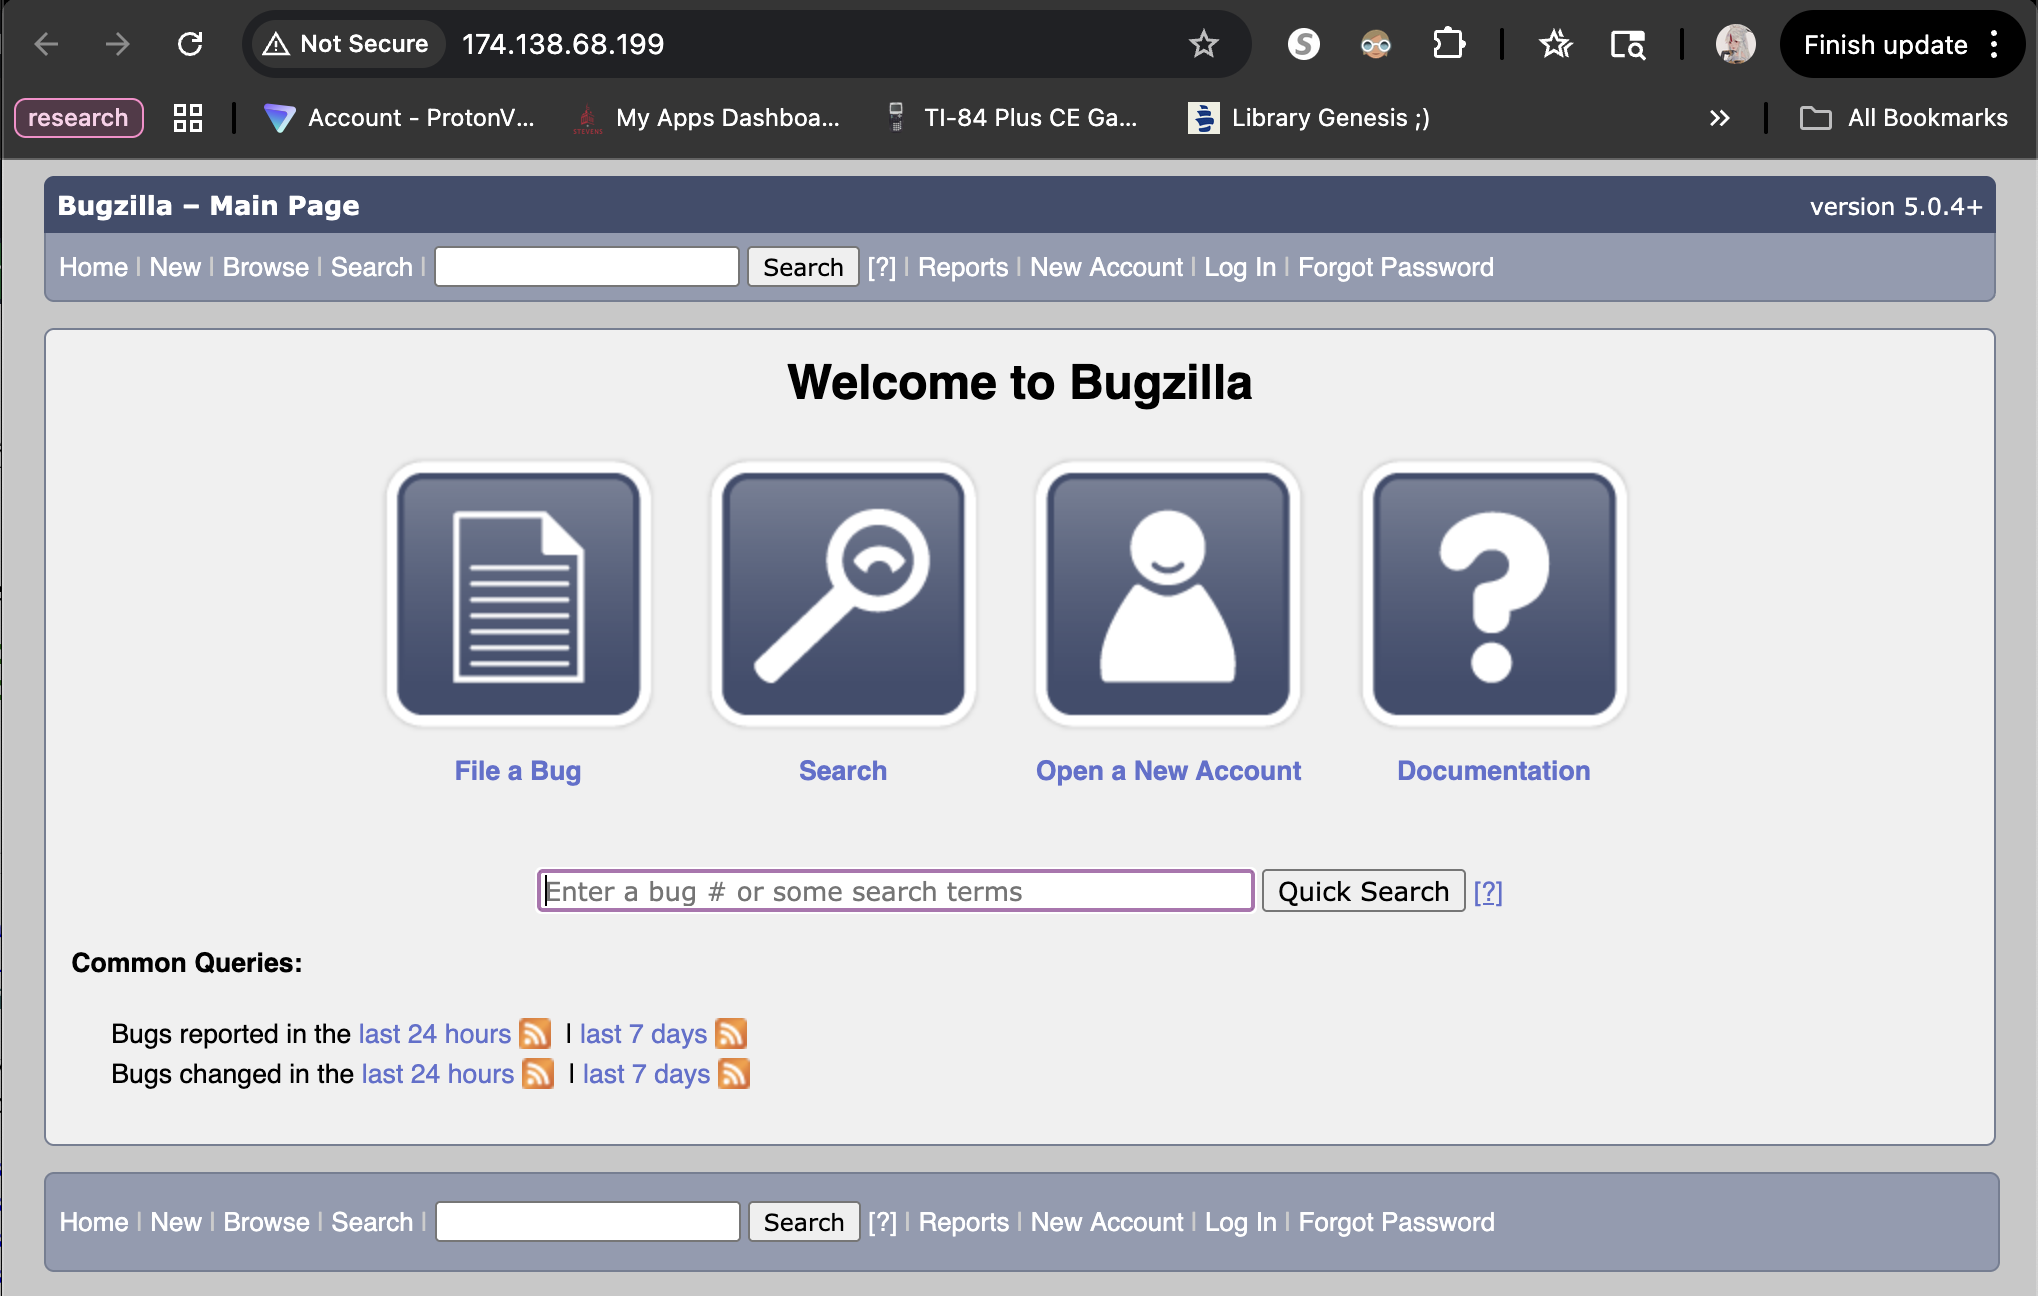
\includegraphics[width=0.7\linewidth]{png/bugzilla_landing.png}
    \caption{bugzilla website on http://174.138.68.199/}
    \label{fig:placeholder}
\end{figure}

\noindent logged in with the given email and password, then head to Administration → Users and re-setted the password and email to real ones.

\noindent and now everything is running on http://174.138.68.199/. :)





\chapter{Overleaf \\
\small{\textit{-- Annanya Jain, Luo Xu, Gavin Lam}
\index{Overleaf} 
\index{Chapter!Overleaf}
\label{Chapter::Overleaf}}}

\title{Deploying Overleaf on a Shared DigitalOcean Droplet (with Existing Bugzilla)}
\section{Overview}
TThis document explains the complete process of deploying \textbf{Overleaf (Community Edition)} on a DigitalOcean droplet that already hosted \textbf{Bugzilla} via Docker.  
It includes the initial access issues, configuration steps, and debugging process that led to a fully functional Overleaf instance running alongside Bugzilla on the same host.

\section{Initial Access Issue}
At the beginning, I could not connect to the droplet from my local machine using its public IP address.  
Both \texttt{ssh root@174.138.68.199} and web requests to \texttt{http://174.138.68.199} were failing with timeout errors.

Since I didn’t originally create the droplet, I did not have SSH access permissions. To resolve this, my teammate who had created the droplet and had root access, added my GitHub SSH key to the droplet’s authorized keys through the DigitalOcean dashboard:

\begin{enumerate}
  \item Logged into \textbf{DigitalOcean}.
  \item Opened the droplet’s page.
  \item Navigated to \textbf{Access → Add SSH Keys}.
  \item Added my GitHub SSH key (fetched automatically from my GitHub account).
\end{enumerate}

After this, I was able to connect successfully:
\begin{minted}[fontsize=\small]{bash}
ssh root@174.138.68.199
\end{minted}

Once connected, I could verify that Bugzilla was already running:
\begin{minted}[fontsize=\small]{bash}
docker ps
\end{minted}

Bugzilla was occupying port 80, so I decided to host Overleaf on a different port.

\section{Overleaf Setup Process}

\subsection{Step 1: Create Project Directory}
\begin{minted}[fontsize=\small]{bash}
mkdir ~/overleaf-docker
cd ~/overleaf-docker
\end{minted}

\subsection{Step 2: Create Environment File}
\begin{minted}[fontsize=\small]{bash}
nano .env
\end{minted}

Contents:
\begin{minted}[fontsize=\small]{text}
OVERLEAF_PORT=8090
OVERLEAF_DOMAIN=http://174.138.68.199:8090
OVERLEAF_ADMIN_EMAIL=(email here)
OVERLEAF_ADMIN_PASSWORD=(password here)
MONGO_INITDB_ROOT_USERNAME=(username here)
MONGO_INITDB_ROOT_PASSWORD=(password here)
\end{minted}

\subsection{Step 3: Write the Docker Compose File}
\begin{minted}[fontsize=\small, bgcolor=gray!5, linenos]{yaml}
version: "3.8"

services:
  mongo:
    image: mongo:6.0
    restart: unless-stopped
    command: ["--replSet", "rs0", "--bind_ip_all"]
    volumes:
      - mongo_data:/data/db

  redis:
    image: redis:7
    restart: unless-stopped

  overleaf:
    image: sharelatex/sharelatex:latest
    restart: unless-stopped
    depends_on:
      - mongo
      - redis
    ports:
      - "8090:80"
    environment:
      OVERLEAF_MONGO_URL: mongodb://mongo:27017/sharelatex?replicaSet=rs0
      OVERLEAF_REDIS_HOST: redis
      OVERLEAF_SITE_URL: http://174.138.68.199:8090
      OVERLEAF_ADMIN_EMAIL: admin@example.com
      OVERLEAF_ADMIN_PASSWORD: password123
      OVERLEAF_APP_NAME: Overleaf
      OVERLEAF_ALLOW_PUBLIC_REGISTRATION: "true"

volumes:
  mongo_data:
\end{minted}


\subsection{Step 4: Launch the Containers}
\begin{minted}[fontsize=\small]{bash}
docker compose up -d
docker ps
\end{minted}

At this point, MongoDB, Redis, and Overleaf containers appeared, but Overleaf was continuously restarting.

\section{Debugging the Overleaf Restart Loop}

\subsection{Step 1: Check Logs}
\begin{minted}[fontsize=\small]{bash}
docker logs overleaf-docker-overleaf-1 --tail 40
\end{minted}

\subsection{Step 2: Error Observed}
\begin{minted}[fontsize=\small]{text}
The MongoDB server has featureCompatibilityVersion=5.0,
but Overleaf requires at least version 6.0.
Aborting.
\end{minted}

\begin{figure}
    \centering
    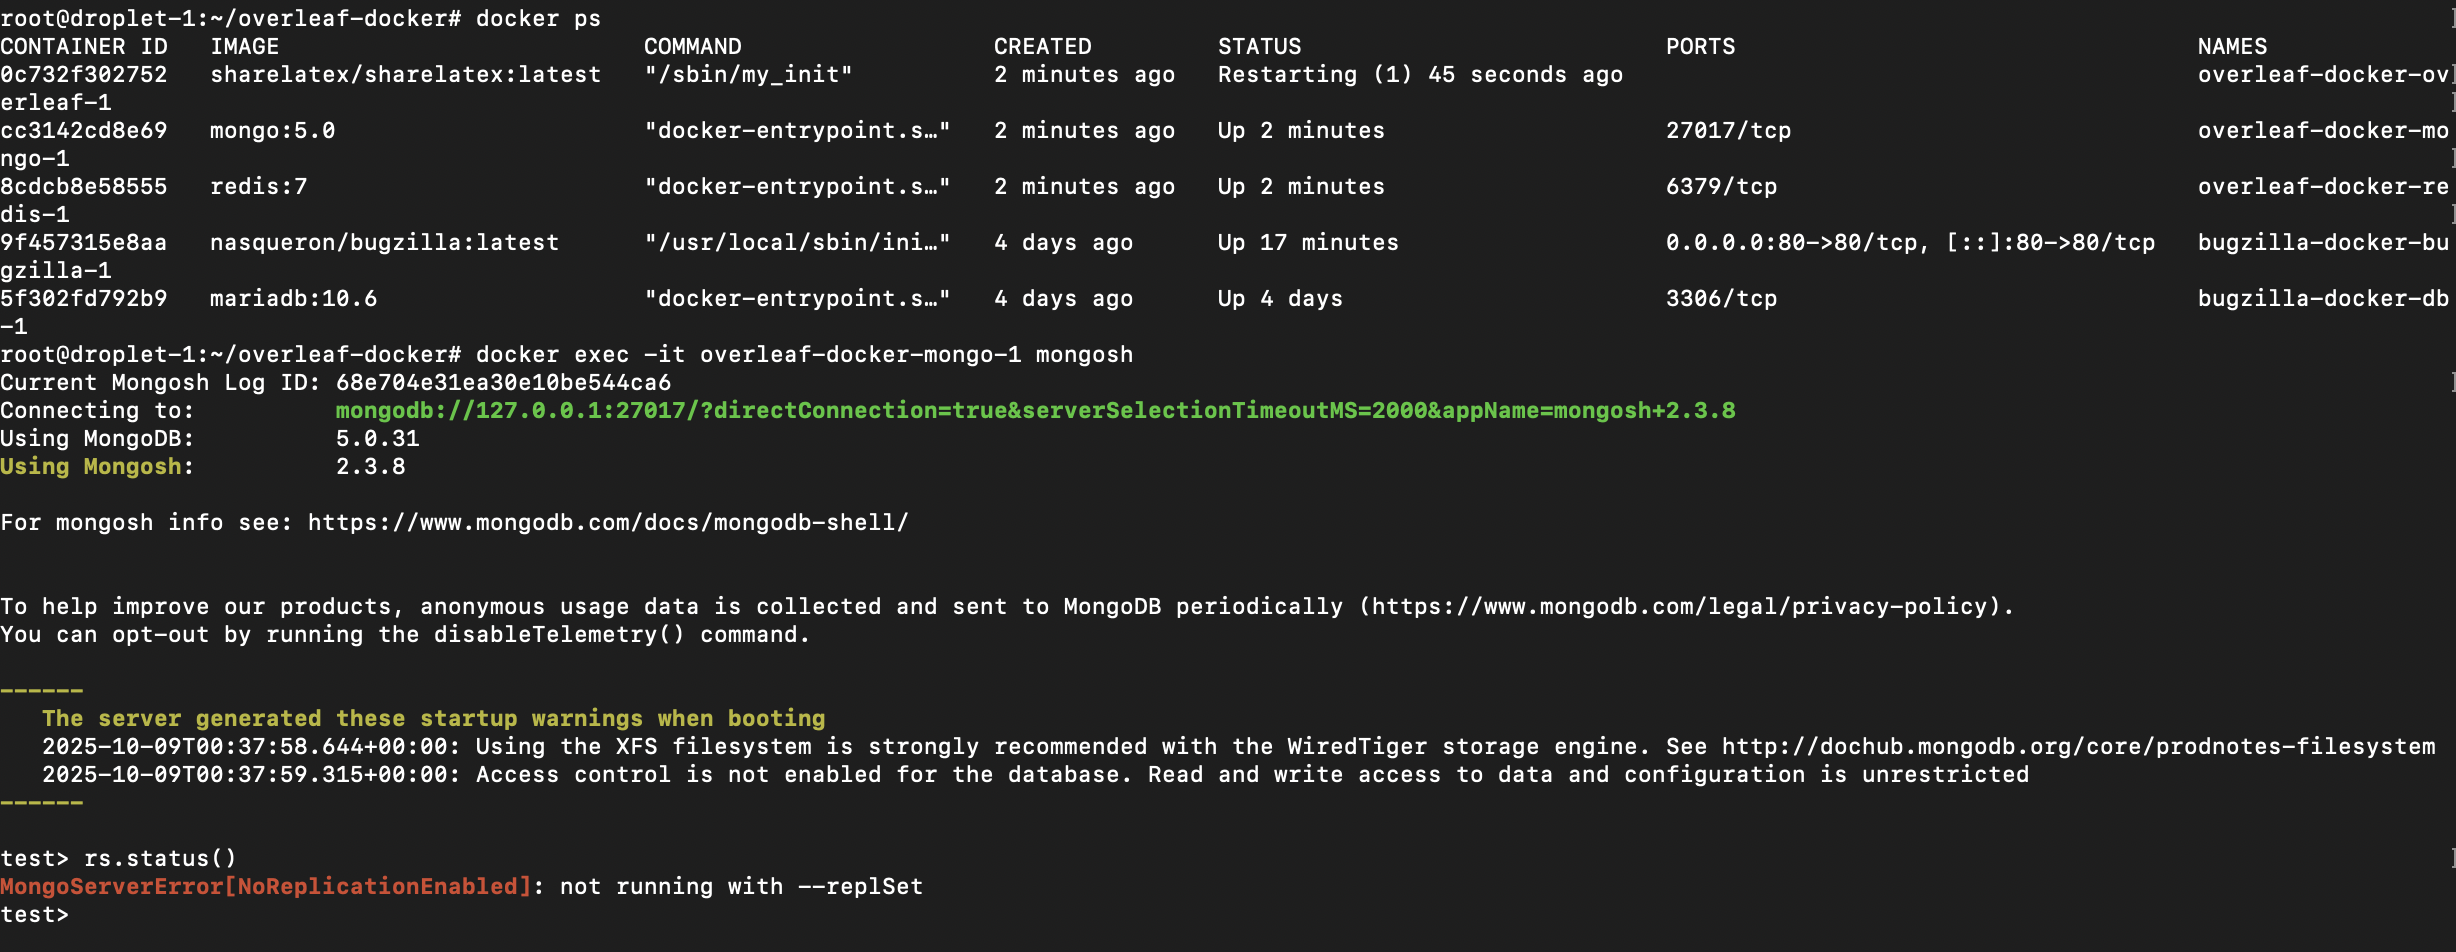
\includegraphics[width=1.0\linewidth]{png/restarting_problem_overleaf.png}
\end{figure}

This indicated that MongoDB was version 6.0, but its internal
\texttt{featureCompatibilityVersion (FCV)} was still set to 5.0.

\section{Fixing MongoDB Configuration}

\subsection{Step 1: Enter Mongo Shell}
\begin{minted}[fontsize=\small]{bash}
docker exec -it overleaf-docker-mongo-1 mongosh
\end{minted}

\subsection{Step 2: Initialize Replica Set}
\begin{minted}[fontsize=\small]{js}
rs.initiate()
\end{minted}

If you see \texttt{MongoServerError[AlreadyInitialized]}, it means it’s already set up — that’s fine.

\subsection{Step 3: Update Feature Compatibility Version}
\begin{minted}[fontsize=\small]{js}
use admin
db.adminCommand({ setFeatureCompatibilityVersion: "6.0" })
\end{minted}

Expected output:
\begin{minted}[fontsize=\small]{json}
{ "ok" : 1 }
\end{minted}

\subsection{Step 4: Restart Overleaf}
\begin{minted}[fontsize=\small]{bash}
exit
docker restart overleaf-docker-overleaf-1
\end{minted}


\section{Making Overleaf Publicly Accessible}

Since Bugzilla was already bound to port 80, Overleaf was assigned to port 8090.  
I confirmed the port was open:
\begin{minted}[fontsize=\small]{bash}
ss -tuln | grep 8090
\end{minted}

Then enabled it in the firewall:
\begin{minted}[fontsize=\small]{bash}
sudo ufw allow 8090/tcp
sudo ufw reload
\end{minted}

\section{Access and Verification}
Once restarted, Overleaf was reachable at:
\begin{minted}[fontsize=\small]{text}
http://174.138.68.199:8090
\end{minted}

I verified it via:
\begin{minted}[fontsize=\small]{bash}
curl -I http://174.138.68.199:8090
\end{minted}

Result:
\begin{minted}[fontsize=\small]{text}
HTTP/1.1 200 OK
\end{minted}

\section{Conclusion on Setting up Overleaf}
The deployment succeeded after:
\begin{enumerate}
  \item Gaining SSH access by adding my GitHub SSH key to the droplet.
  \item Running Overleaf on port 8090 (to avoid conflict with Bugzilla on port 80).
  \item Initializing the MongoDB replica set.
  \item Updating the MongoDB feature compatibility version to 6.0.
\end{enumerate}

After these steps, Overleaf was fully functional and accessible publicly via:
\begin{minted}[fontsize=\small]{text}
http://174.138.68.199:8090
\end{minted}

\begin{figure}
    \centering
    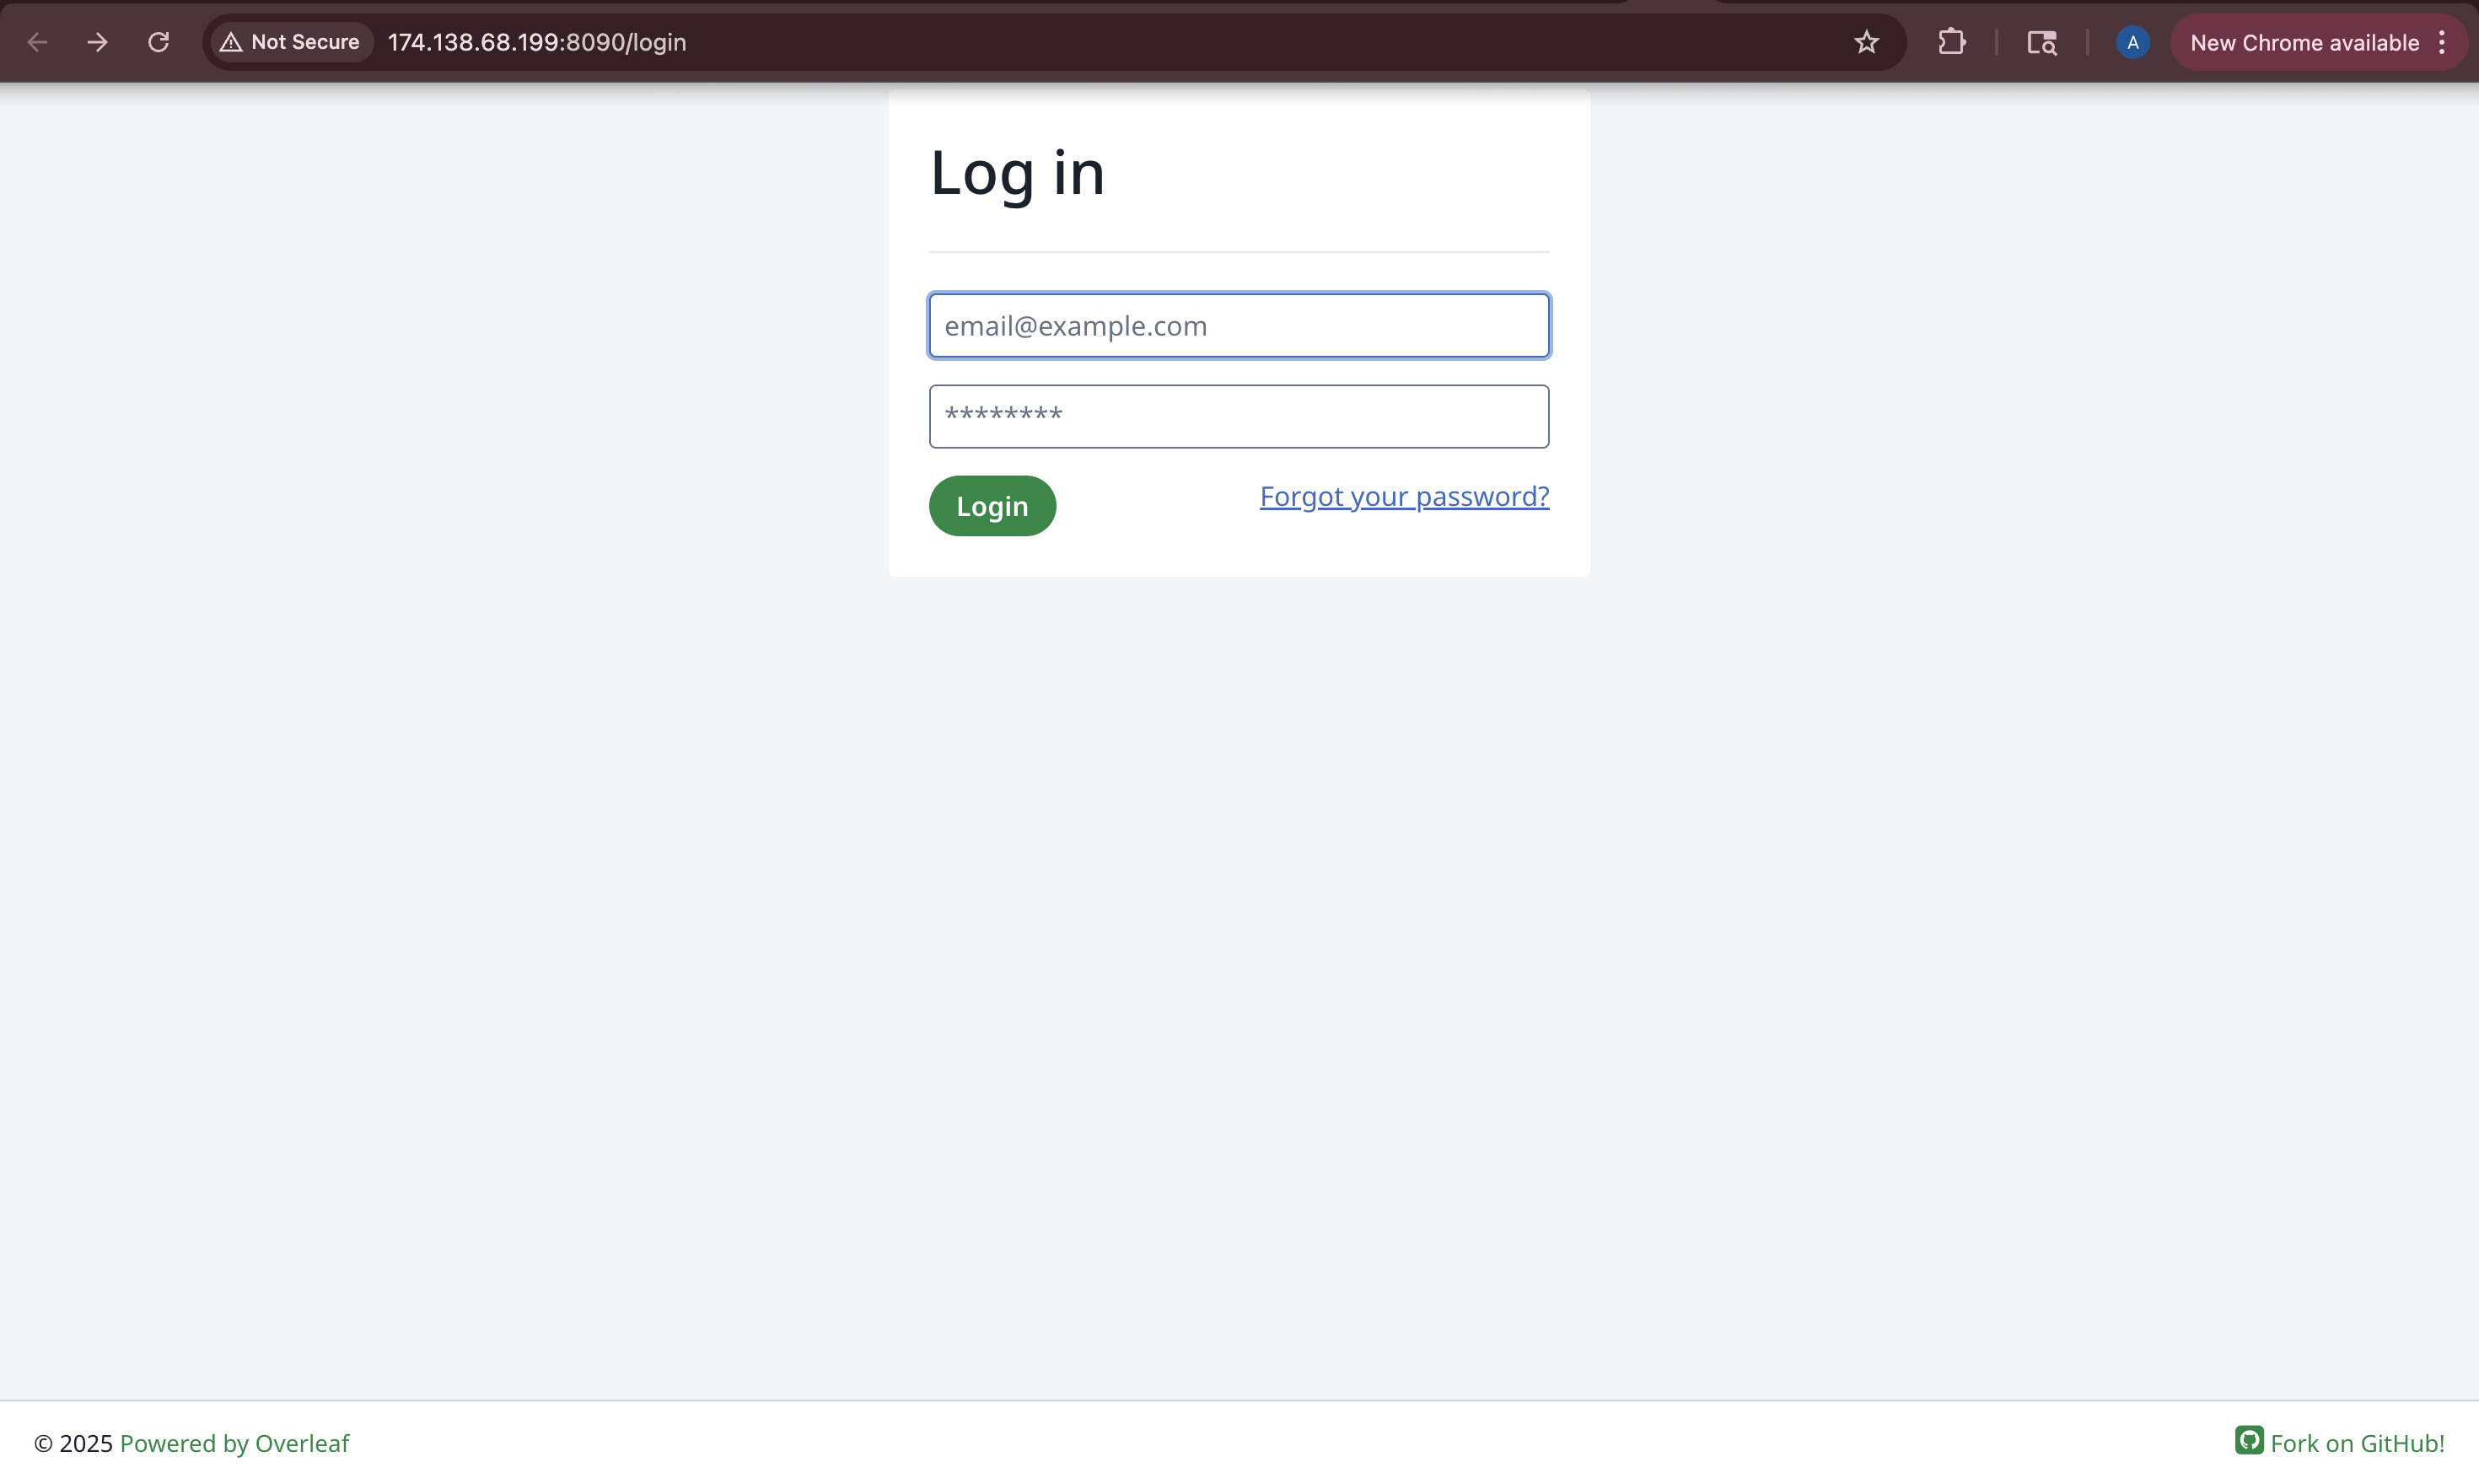
\includegraphics[width=1.0\linewidth]{png/overleaf running.png}
    \caption{overleaf website on http://174.138.68.199:8090}
    \label{fig:placeholder}
\end{figure}

This was what was seen:
\begin{figure}
    \centering
    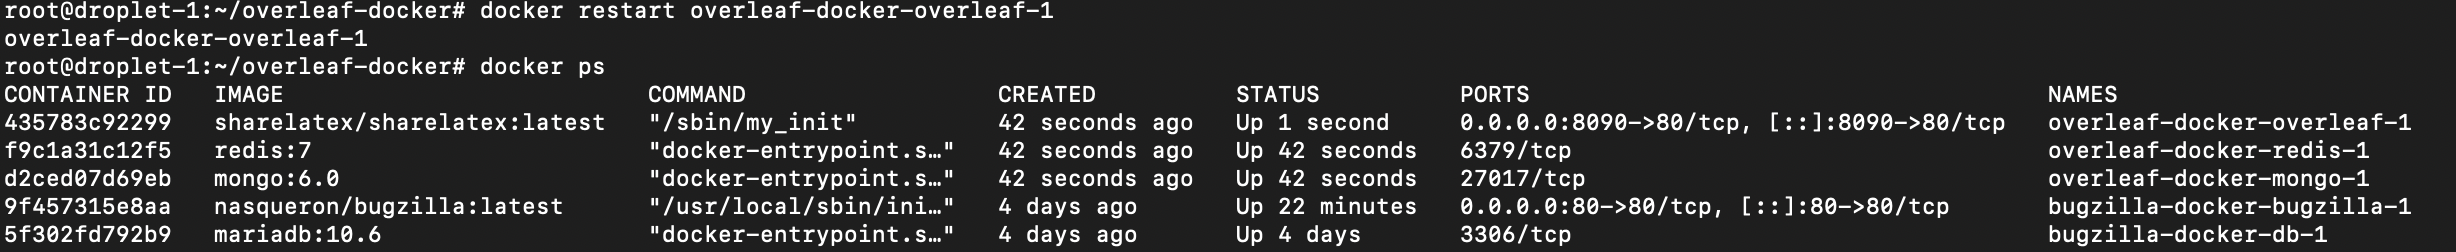
\includegraphics[width=1.0\linewidth]{png/finally_fixed.png}
\end{figure}

\section{Setting up Overleaf Packages}
Even thought Overleaf is up and running, we weren't able to run our document due to Overleaf not having access to any of the packages we were using. Thus we had to download the packages needed with commands:
\begin{minted}{bash}
apt-get update
apt-get install -y texlive-full
mktexlsr
\end{minted}
This took a long time to run, but afterwards our notebook was able to compile and had no errors in showing the pdf, however minted has refused to work even after installation...

\section{Connection Our Overleaf Instance to GitHub}
I first created a new GitHub Repository to for Overleaf, and then connected to our droplet. I downloaded the zip file for the Overleaf, then I copied it over to the vm and unzipped it under the repo. 

\appendix
\chapter{Appendix \\
\small{\textit{-- Gavin Lam, Spurthi Setty, Annanya Jain, Luo Xu}}
\index{appendix} 
\index{Chapter!Appendix}
\label{Chapter::Appendix}}

% makeglossaries dsnManual -- from command prompt.
\clearpage
%\printglossaries


\printnoidxglossaries

\bibliography{bibfile}
%\bibliographystyle{unsrt}
\bibliographystyle{IEEEtran}

\printindex
%\input{dsnManual.idx}
\end{document}
